\documentclass[11pt,a4paper]{article}

% ── Packages ──────────────────────────────────────────────────────────────────
\usepackage[T1]{fontenc}
\usepackage[utf8]{inputenc}
\usepackage{helvet}
\renewcommand{\familydefault}{\sfdefault}   % Arial-like sans-serif font
\usepackage[margin=2.5cm]{geometry}
\usepackage{hyperref}
\usepackage{listingsutf8}
\usepackage{xcolor}
\usepackage{enumitem}
\usepackage{titlesec}
\usepackage{parskip}
\usepackage{booktabs}
\usepackage{graphicx}
\usepackage{amsmath}
\usepackage{fancyhdr}
\usepackage[title]{appendix}
\usepackage{tikz}
\usetikzlibrary{shapes.geometric, arrows.meta, positioning, fit, backgrounds}

% ── Colors ────────────────────────────────────────────────────────────────────
\definecolor{codebg}{HTML}{F5F5F5}
\definecolor{codeframe}{HTML}{CCCCCC}
\definecolor{keyword}{HTML}{0000CC}
\definecolor{comment}{HTML}{007700}
\definecolor{string}{HTML}{CC0000}
\definecolor{uu-red}{HTML}{990000}

% ── Listings style ────────────────────────────────────────────────────────────
\lstdefinestyle{docker}{
  language=bash,
  basicstyle=\ttfamily\small,
  backgroundcolor=\color{codebg},
  frame=single,
  rulecolor=\color{codeframe},
  breaklines=true,
  breakatwhitespace=true,
  columns=fullflexible,
  keepspaces=true,
  showstringspaces=false,
  commentstyle=\color{comment},
  keywordstyle=\color{keyword}\bfseries,
  stringstyle=\color{string},
  numbers=left,
  numberstyle=\tiny\color{gray},
  numbersep=8pt,
  tabsize=2,
}

\lstdefinestyle{yaml}{
  language=bash,
  basicstyle=\ttfamily\small,
  backgroundcolor=\color{codebg},
  frame=single,
  rulecolor=\color{codeframe},
  breaklines=true,
  columns=fullflexible,
  keepspaces=true,
  showstringspaces=false,
  morecomment=[l]{\#},
  commentstyle=\color{comment},
  numbers=left,
  numberstyle=\tiny\color{gray},
  numbersep=8pt,
  tabsize=2,
}

\lstdefinestyle{shell}{
  language=bash,
  basicstyle=\ttfamily\small,
  backgroundcolor=\color{codebg},
  frame=single,
  rulecolor=\color{codeframe},
  breaklines=true,
  columns=fullflexible,
  keepspaces=true,
  showstringspaces=false,
}

\lstdefinestyle{python}{
  language=Python,
  basicstyle=\ttfamily\small,
  backgroundcolor=\color{codebg},
  frame=single,
  rulecolor=\color{codeframe},
  breaklines=true,
  breakatwhitespace=true,
  columns=fullflexible,
  keepspaces=true,
  showstringspaces=false,
  commentstyle=\color{comment},
  keywordstyle=\color{keyword}\bfseries,
  stringstyle=\color{string},
  numbers=left,
  numberstyle=\tiny\color{gray},
  numbersep=8pt,
  tabsize=4,
}

% ── Section title formatting ──────────────────────────────────────────────────
\lstset{inputencoding=utf8, extendedchars=true}
\titleformat{\section}{\large\bfseries\color{black}}{\thesection}{1em}{}
\titleformat{\subsection}{\normalsize\bfseries}{\thesubsection}{1em}{}

% ── Header / Footer ───────────────────────────────────────────────────────────
\pagestyle{fancy}
\fancyhf{}
\lhead{\small Data Engineering II -- Assignment 3}
\rhead{\small Uppsala University}
\cfoot{\thepage}

% ── Hyperref setup ────────────────────────────────────────────────────────────
\hypersetup{
  colorlinks=true,
  linkcolor=black,
  urlcolor=blue,
}

% ─────────────────────────────────────────────────────────────────────────────
\begin{document}

% ── Title page ────────────────────────────────────────────────────────────────
\begin{titlepage}
  \centering
  \vspace*{2cm}
  {\large Uppsala University\\[0.3em]
   Department of Information Technology\\[2cm]}
  {\LARGE\bfseries Assignment 3\\[0.5em]}
  {\Large Distributed Infrastructure, Model Serving and CI/CD\\[2cm]}
  {\large Course: Data Engineering II\\[1.5cm]}
  {\normalsize Arnab Kumar Ghosh\\[0.5cm]}
  {\normalsize \today\\[3cm]}
  \vfill
\end{titlepage}

\tableofcontents
\newpage

% =============================================================================
\section{Introduction}
% =============================================================================

This assignment covers the deployment of a distributed machine learning application
across a cloud infrastructure. Assignment 3 consists of four progressive tasks.
Task 1 starts with a single server deployed to a single virtual machine using CloudInit for contextualization.
Task 2 improves this by containerizing services with Docker and Docker Compose.
Task 3 adds multi-server orchestration using Ansible.
Task 4 completes the setup with a continuous deployment pipeline using Git hooks.
Each task builds on the previous one, introducing new tools and addressing
previous limitations.

% =============================================================================
\section{Task 1: Single Server Deployment}
% =============================================================================

\subsection{Overview}

Task 1 requires deploying a machine learning model serving application on a single
virtual machine using CloudInit for dynamic contextualization. The application
consists of three components: a Flask web frontend, a Celery worker, and a RabbitMQ
message broker. The model is a Keras/TensorFlow neural network trained on the Pima
Indians Diabetes dataset. The deployment must be automated from a client VM using the OpenStack Python API.
During the first boot, CloudInit is responsible for all software installation and
service startup. This eliminates the need for any manual login to the production server.

\subsection{Application Architecture}

The production server has three components:

\begin{itemize}[leftmargin=1.5cm]
  \item \textbf{Flask app} (\texttt{app.py}): runs the web frontend on port 5100.
        It receives prediction requests from the browser and sends them to Celery
        as tasks.
  \item \textbf{RabbitMQ}: sits between Flask and Celery. It holds tasks in a queue
        until a worker is ready.
  \item \textbf{Celery worker} (\texttt{workerA.py}): takes a task from the queue,
        loads the Keras model, runs the prediction, and sends the result back.
\end{itemize}

The data flow is:
\begin{center}
  \texttt{Browser} $\rightarrow$ \texttt{Flask (app.py)} $\rightarrow$
  \texttt{RabbitMQ} $\rightarrow$ \texttt{Celery worker (workerA.py)}
  $\rightarrow$ \texttt{Flask} $\rightarrow$ \texttt{Browser}
\end{center}

\subsection{CloudInit Configuration}

The file \texttt{cloud-cfg.txt} is given to OpenStack when the production VM is
created. CloudInit runs the steps below automatically on the first boot:

\begin{lstlisting}[style=yaml, caption={cloud-cfg.txt -- single server without Docker}]
#cloud-config

apt_update: true
apt_upgrade: true
packages:
 - python3-pip
 - python3-dev
 - build-essential
 - rabbitmq-server

byobu_default: system

runcmd:
 - pip3 install "celery" "tensorflow==2.10.0" "amqp" "flask==2.3.1" "future" "numpy<2.0"
 - git clone https://github.com/sztoor/model_serving.git
 - celery --workdir=/model_serving/single_server_without_docker/production_server \
       -A workerA worker --detach --loglevel=debug --concurrency=1 -n wkr1@backend
 - python3 /model_serving/single_server_without_docker/production_server/app.py \
       --host=0.0.0.0 --port=5100 &
\end{lstlisting}

\subsection{Starting the Production VM}

On the client VM, I sourced the OpenStack RC file and installed the OpenStack Python
libraries. Then I ran the following command:

\begin{lstlisting}[style=shell, caption={Starting the production VM from the client}]
python3 start_instance.py
\end{lstlisting}

The script read credentials from the environment, created the VM with the
CloudInit user-data, and waited until the instance status was \texttt{ACTIVE}.
After I attached a floating IP, the application was reachable at:

\begin{itemize}[leftmargin=1.5cm]
  \item Welcome page: \texttt{http://130.238.27.96:5100}
  \item Predictions page: \texttt{http://130.238.27.96:5100/predictions}
\end{itemize}

\subsection{Questions}

\subsubsection*{1. Explain how the application works.}

The application has three tiers. A client sends input values to the Flask web page.
Flask puts the prediction request into a RabbitMQ queue as a Celery task. A Celery
worker picks up the task, loads the model from \texttt{model.h5} and
\texttt{model.json}, runs the prediction, and saves the result. Flask then reads
the result and shows it on the \texttt{/predictions} page. This design keeps the
web server fast because heavy model computation runs in a separate worker process.

\subsubsection*{2. What are the drawbacks of the contextualization strategy adopted in Task 1?}

\begin{enumerate}[leftmargin=1.5cm]
  \item \textbf{Slow deployment}: every new VM must download and install all
        packages from the internet at boot time. This takes 10--15 minutes.
  \item \textbf{No reproducibility}: the script runs \texttt{apt\_upgrade: true},
        so the latest package versions are installed. A new VM created later may get
        different package versions and behave differently.
  \item \textbf{No isolation}: all services share the same OS. A package conflict
        or a crashed service can bring down the whole server.
  \item \textbf{No automatic restart}: services are started as background processes.
        If a process crashes, nothing restarts it.
  \item \textbf{Hard to scale}: adding a Celery worker requires logging in to the VM
        and running commands manually. There is no automated way to scale.
  \item \textbf{No persistence}: if the VM is deleted, all data and configuration
        are lost. The whole setup must be done again from scratch.
\end{enumerate}

\subsubsection*{3. How can we reduce the deployment time?}

Most of the time is spent downloading and installing packages on each new VM.
A pre-built Docker image solves this. All dependencies are installed once and
saved to an image registry. When the VM boots, it only pulls the image and starts
a container. This takes seconds instead of minutes. Another option is to create
a custom OpenStack snapshot with all packages already installed. The VM then boots
from that snapshot and skips the \texttt{apt install} step entirely.

\subsubsection*{4. Summary}

In this task, I deployed a complete machine learning serving stack to a fresh cloud
VM with no manual intervention after the VM was created. The only input I provided
was a single \texttt{cloud-cfg.txt} file passed to the OpenStack API at launch time.

I sourced the OpenStack RC file on the client VM and ran \texttt{start\_instance.py},
which called the OpenStack API to create the production VM.
CloudInit then executed automatically on the first boot. It updated the system
packages and installed Python 3, RabbitMQ, and all required pip packages. It then
cloned the application repository from GitHub and started both the Celery worker
(as a background process) and the Flask web server on port~5100. The entire process from VM creation to a live
service took approximately 12--15~minutes without any further input from me.

I attached  a floating IP and verified that the three-component architecture---Flask, RabbitMQ, and
Celery---worked correctly from the first boot. I submitted input values on the
predictions page. They were queued as a Celery task and processed by the worker using
the Keras model. The prediction result then appeared on the \texttt{/predictions} page. I did not need to
start or configure any service manually after the VM became active.

Despite the successful deployment, I observed several important limitations.
Packages are downloaded and installed at every new boot. This makes deployment slow
and non-reproducible, since different package versions may be installed on different
days.
Since services run as raw background processes with no process supervisor, a crash
is never recovered automatically. All three components share the same OS environment,
meaning a dependency conflict or a bad package upgrade can bring down everything at
once. To scale, I would have to log in to the VM and start workers by hand.

These problems motivated me to move to Docker containers in Task~2, which provides
isolation, automatic restart, and one-command horizontal scaling.

\begin{figure}[htbp]
  \centering
  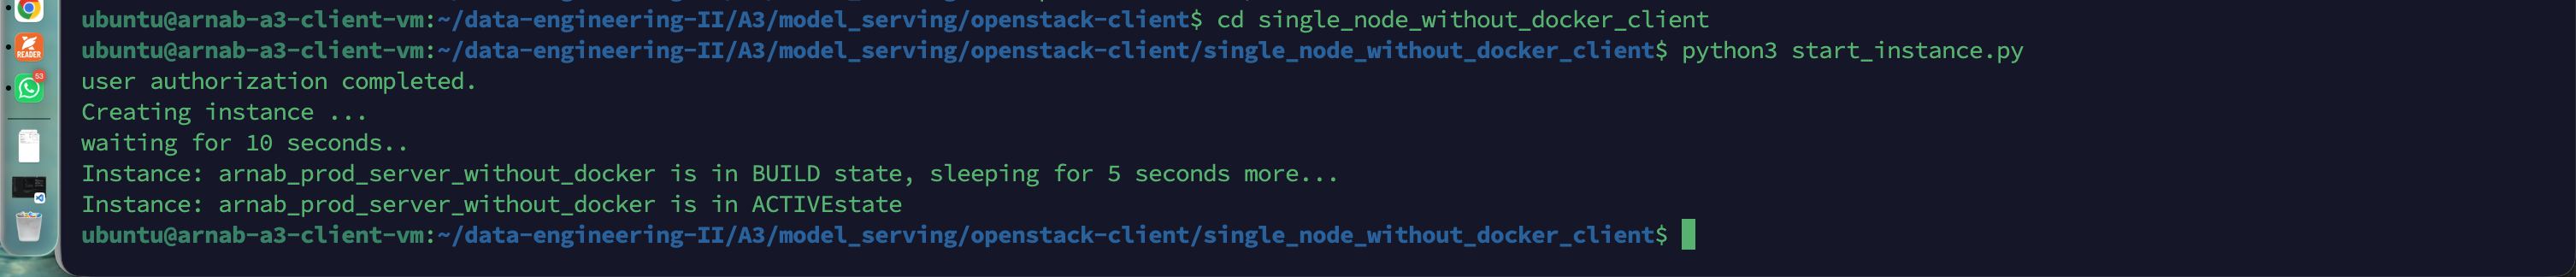
\includegraphics[width=\textwidth]{figure/task-1-start-instance.png}
  \caption{Client VM running \texttt{start\_instance.py} to create the production
           VM via the OpenStack Python API. The script waits until the instance
           status reaches \texttt{ACTIVE} before returning.}
  \label{fig:task1-start}
\end{figure}

\begin{figure}[htbp]
  \centering
  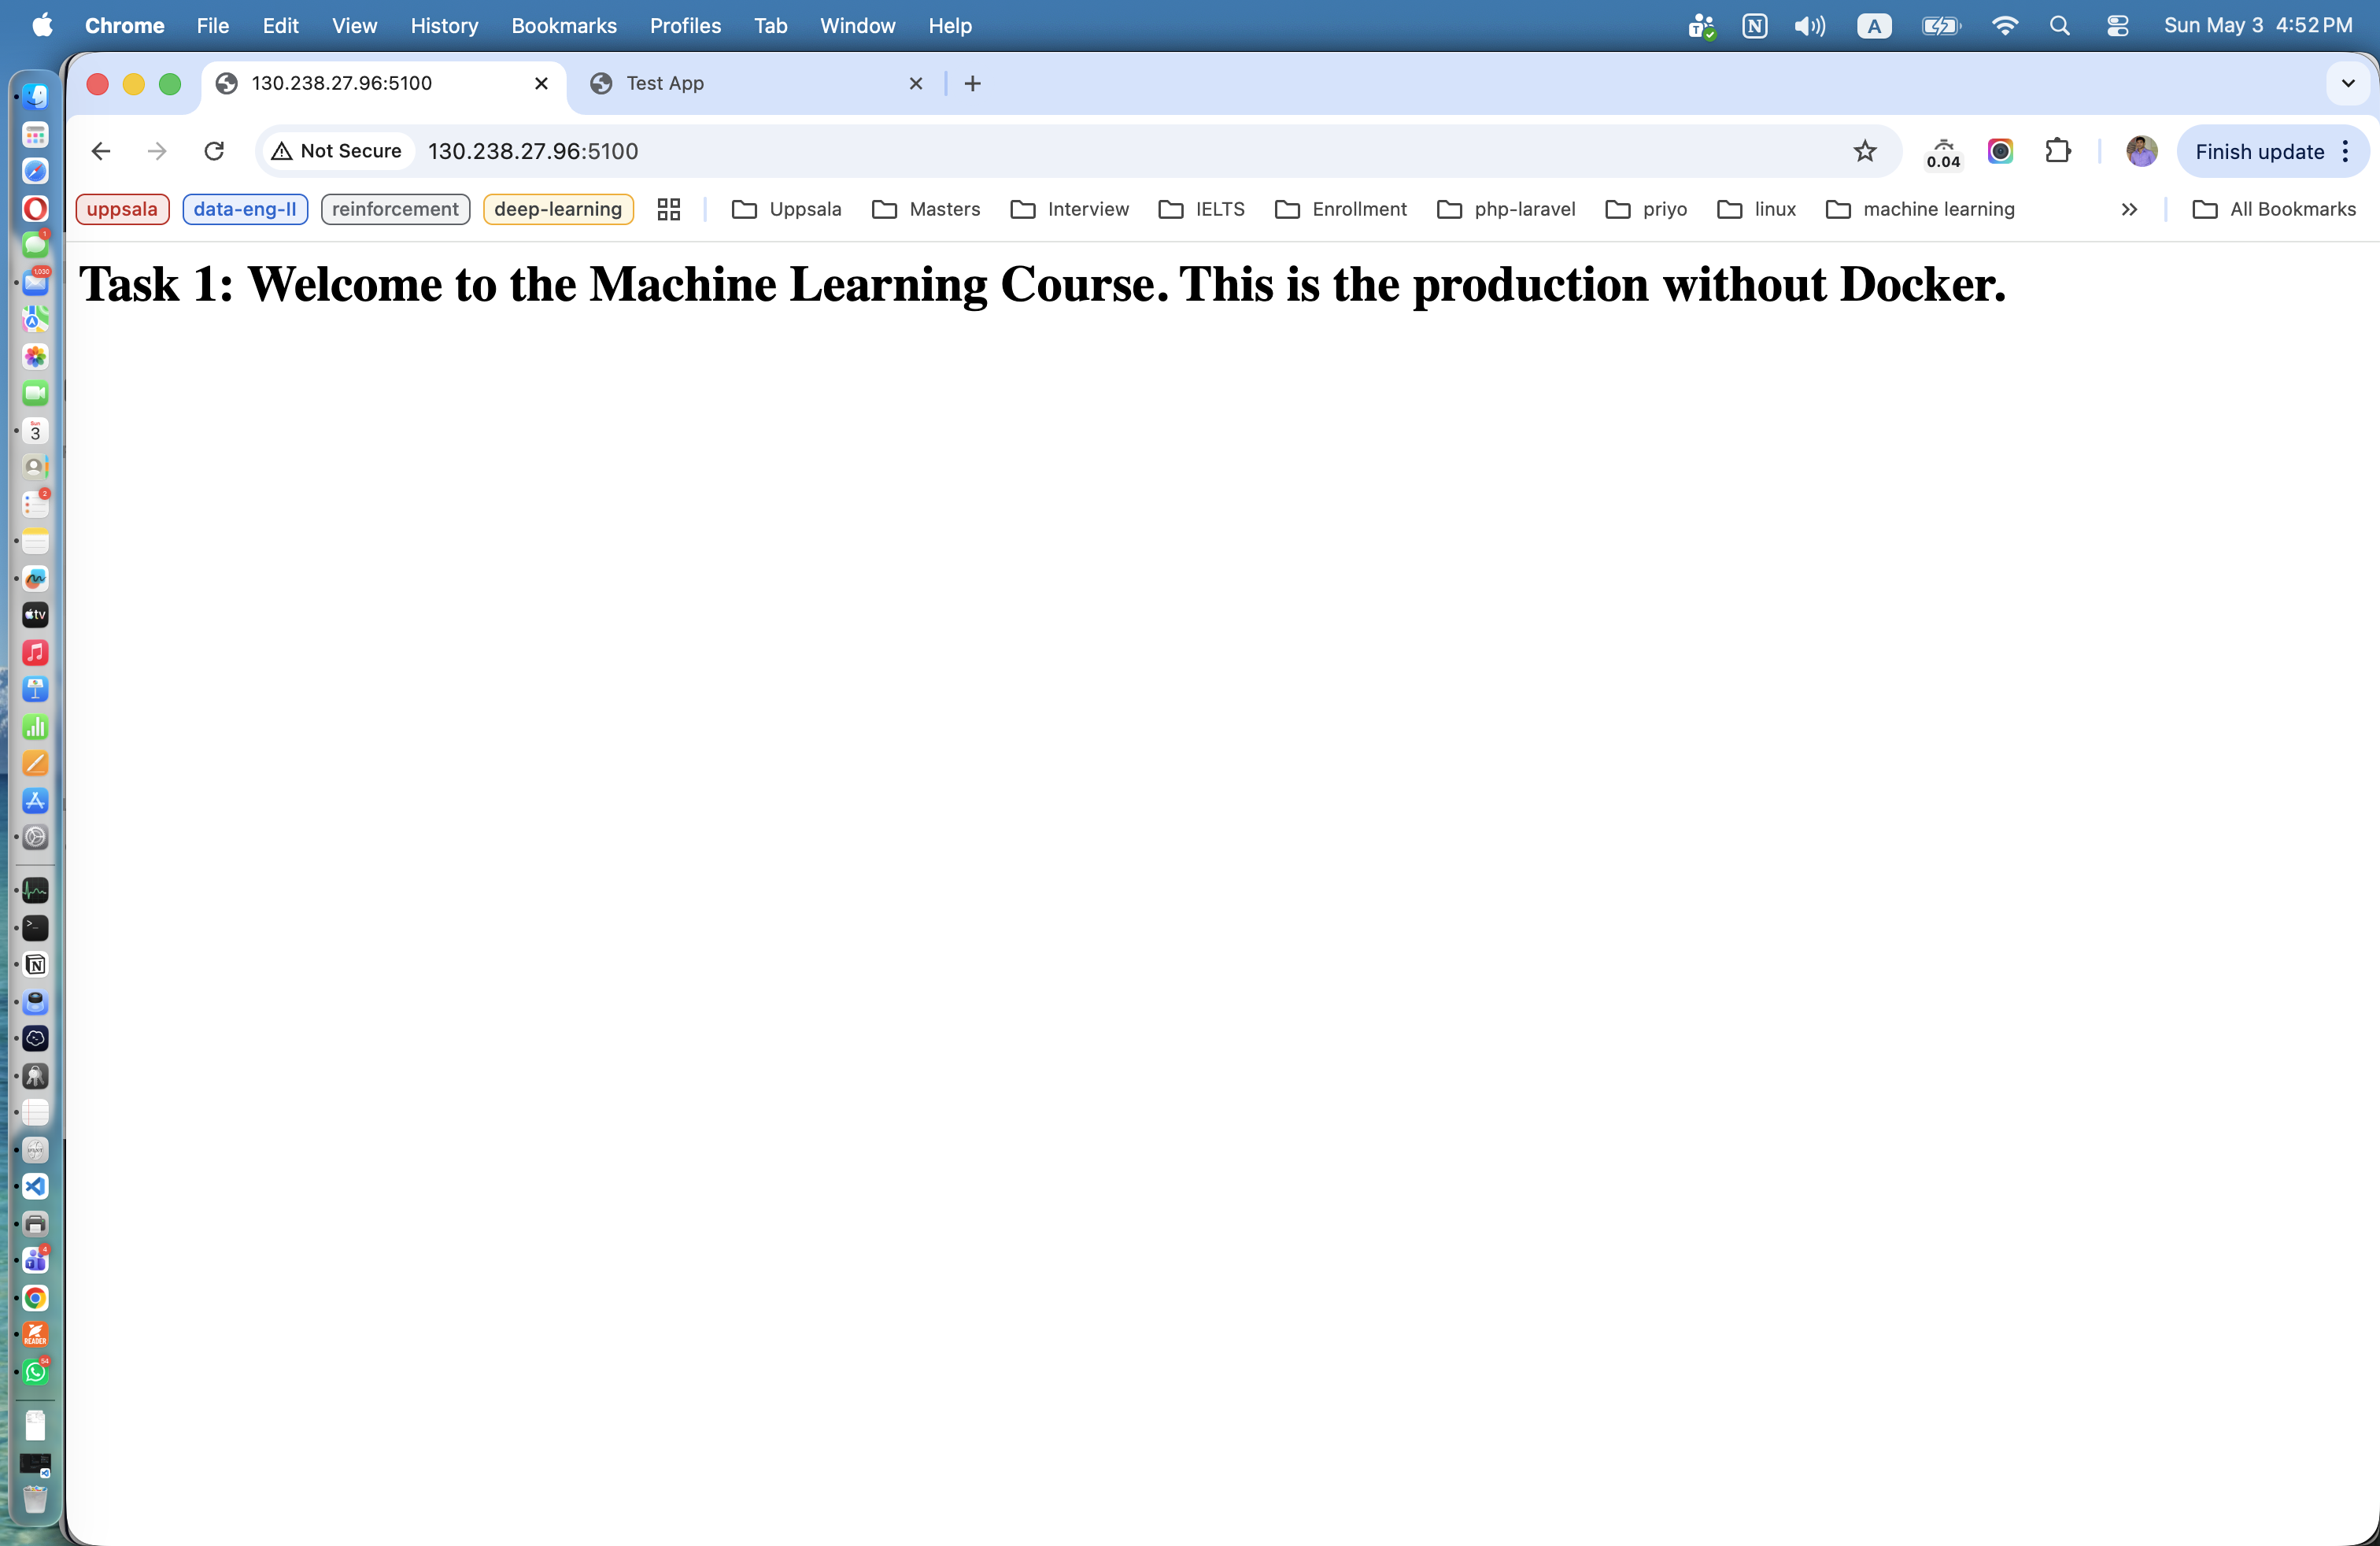
\includegraphics[width=\textwidth]{figure/task-1-welcome.png}
  \caption{Welcome page of the Flask application served on port~5100 after
           CloudInit completed all installation and startup steps.}
  \label{fig:task1-welcome}
\end{figure}

\begin{figure}[htbp]
  \centering
  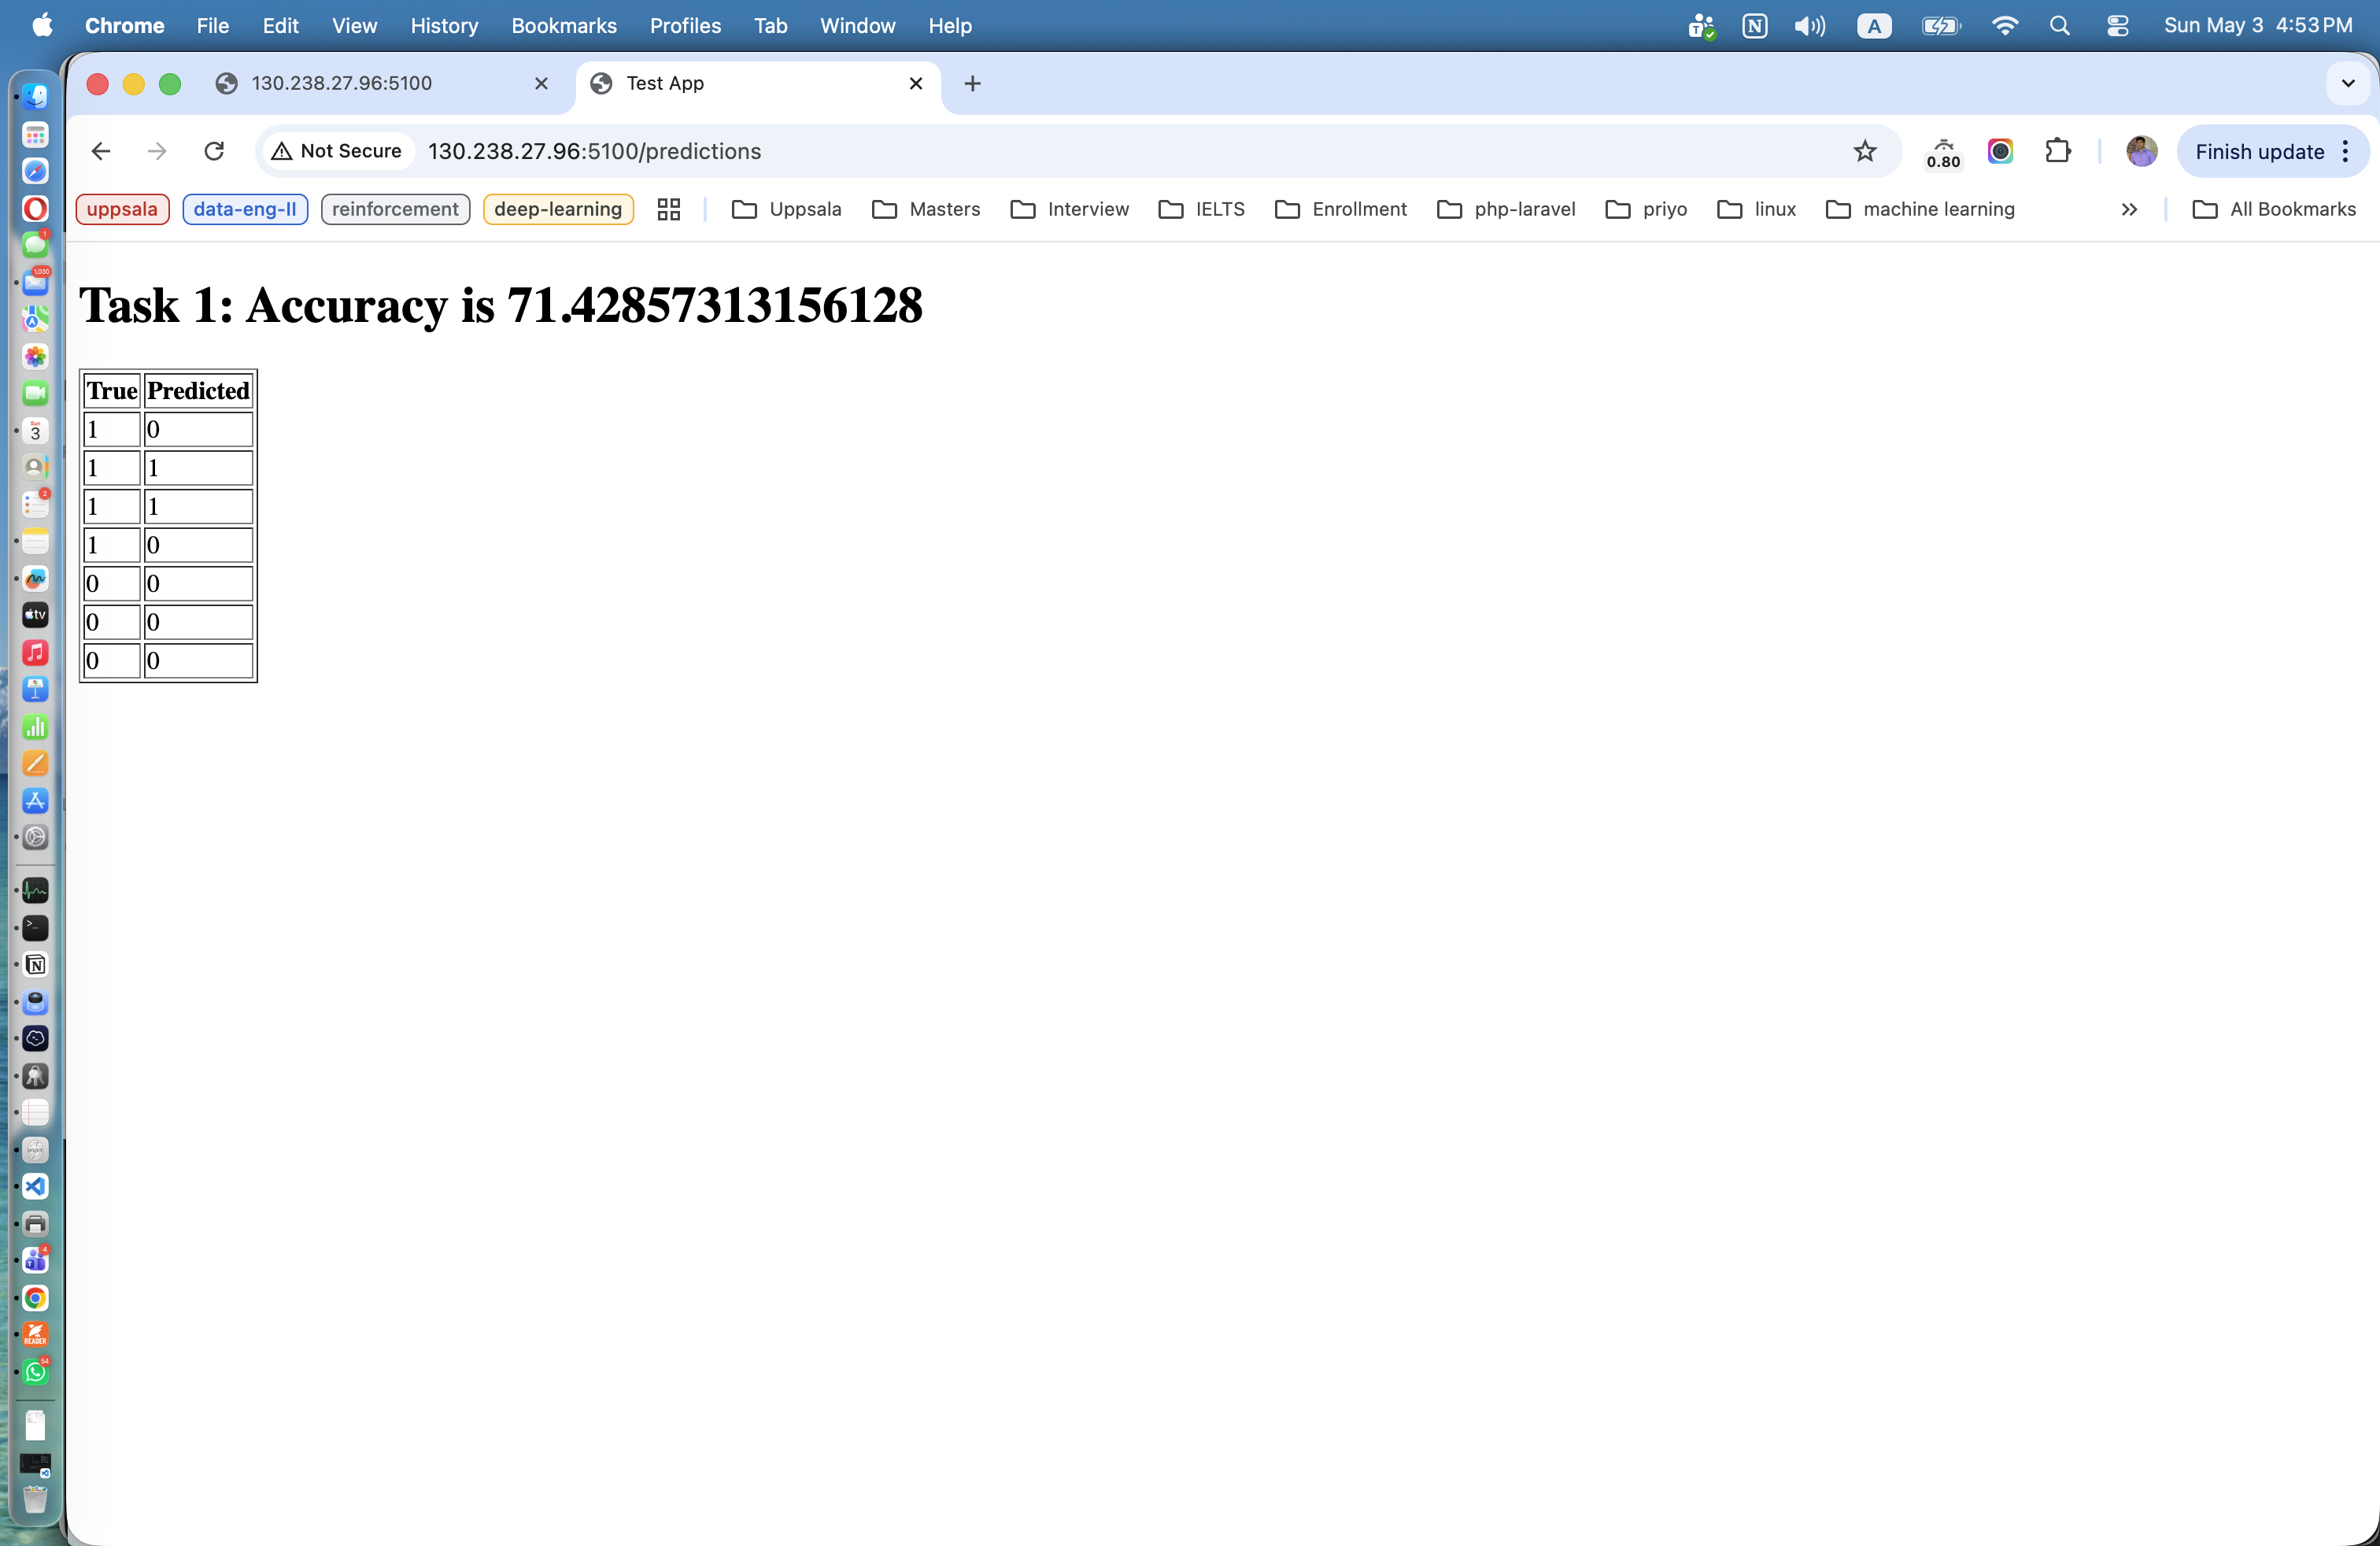
\includegraphics[width=\textwidth]{figure/task-1-predictions.png}
  \caption{Predictions page showing a diabetes prediction result returned by the
           Celery worker via RabbitMQ. The result confirms end-to-end task
           queueing and model inference are working correctly.}
  \label{fig:task1-predictions}
\end{figure}
\newpage
% =============================================================================
\section{Task 2: Single Server Deployment with Docker Containers}
% =============================================================================

\subsection{Overview}

Task 2 requires repeating the deployment from Task 1, but replacing direct package
installation with Docker and Docker Compose. Each service must run in its own
isolated container built from a Dockerfile. The task also requires
demonstrating horizontal scaling by adding and removing Celery worker containers
with a single command, without modifying Flask or RabbitMQ.

\subsection{Docker Compose Architecture}

The \texttt{docker-compose.yml} defines three services:

\begin{lstlisting}[style=yaml, caption={docker-compose.yml for the production server}]
version: "3"
services:
  web:
    build:
      context: .
      network: host
    restart: always
    ports:
      - "5100:5100"
    depends_on:
      - rabbit
  rabbit:
    hostname: rabbit
    image: rabbitmq:3.11-management
    environment:
      - RABBITMQ_DEFAULT_USER=rabbitmq
      - RABBITMQ_DEFAULT_PASS=rabbitmq
    ports:
      - "5672:5672"
      - "15672:15672"
  worker_1:
    build:
      context: .
      network: host
    hostname: worker_1
    entrypoint: celery
    command: -A workerA worker --loglevel=debug
    links:
      - rabbit
    depends_on:
      - rabbit
\end{lstlisting}

\begin{itemize}[leftmargin=1.5cm]
  \item \textbf{web}: the Flask frontend, built from the local \texttt{Dockerfile}.
        It listens on port 5100 and waits for RabbitMQ to start first.
  \item \textbf{rabbit}: the official RabbitMQ image with the management plugin.
        The login credentials are set through environment variables.
  \item \textbf{worker\_1}: the Celery worker, built from the same \texttt{Dockerfile}
        but started with the Celery command instead of Flask.
\end{itemize}

\subsection{CloudInit Configuration (with Docker)}

The \texttt{cloud-cfg.txt} for this task installs Docker CE and starts the
application with Docker Compose at boot time. Python packages are no longer
installed directly on the VM:

\begin{lstlisting}[style=yaml, caption={cloud-cfg.txt -- single server with Docker}]
#cloud-config
apt_update: true
apt_upgrade: true
packages:
 - apt-transport-https
 - ca-certificates
 - curl
 - software-properties-common
runcmd:
 - curl -fsSL https://download.docker.com/linux/ubuntu/gpg | sudo apt-key add -
 - add-apt-repository -y "deb [arch=amd64] https://download.docker.com/linux/ubuntu focal stable"
 - apt-get update -y
 - apt-get install -y docker-ce
 - git clone https://github.com/sztoor/model_serving.git
 - docker compose -f /model_serving/single_server_with_docker/production_server/docker-compose.yml up -d
\end{lstlisting}

\subsection{Scaling the Workers}

Horizontal scaling was tested on the production VM after deployment.

\begin{lstlisting}[style=shell, caption={Scaling Celery workers from 1 to 3}]
# Initial state -- one worker
sudo docker ps

# Scale up to 3 workers
sudo docker compose up --scale worker_1=3 -d

# Verify three workers are running
sudo docker ps

# Scale back down
sudo docker compose up --scale worker_1=1 -d
\end{lstlisting}

With three workers, five containers were running at the same time:
\texttt{rabbit}, \texttt{web}, \texttt{worker\_1\_1}, \texttt{worker\_1\_2}, and
\texttt{worker\_1\_3}. No changes were needed in Flask or RabbitMQ to add the
extra workers.

\subsection{Questions}

\subsubsection*{1. What problems Task 2 deployment strategy solves compared to the strategy adopted in
Task 1?}

Docker fixes several problems from Task 1. Each service runs in its own container,
so there are no dependency conflicts between Flask, Celery, and RabbitMQ. The
\texttt{restart: always} setting means the web container restarts on its own if it
crashes. Adding workers takes one command with \texttt{--scale}. The \texttt{Dockerfile}
fixes the exact build environment, so the deployment is more reproducible than
installing packages directly with \texttt{pip}.

\subsubsection*{2. What are the outstanding issues that the deployment strategy of Task 2 cannot not
address?}

\begin{itemize}[leftmargin=1.5cm]
  \item \textbf{Single point of failure}: all containers run on one VM. If that VM
        goes down, the whole application stops.
  \item \textbf{No cross-node scaling}: Docker Compose cannot spread containers
        across several VMs. All workers share the resources of one machine.
  \item \textbf{Manual deployment}: a new version requires running
        \texttt{docker compose up} by hand. There is no automated pipeline.
  \item \textbf{No load balancing}: the web service has one container. High traffic
        cannot be spread across multiple web replicas automatically.
\end{itemize}

\subsubsection*{3. What are the possible solutions to address those outstanding issues?}

A container orchestrator such as \textbf{Kubernetes} or \textbf{Docker Swarm} can
run containers on many VMs, restart failed containers, and deploy updates without
downtime. A CI/CD tool such as Git Hooks (Task 4) or GitHub Actions can rebuild and
redeploy the application automatically when code changes. A
load balancer placed in front of several \texttt{web} containers can spread traffic
across all of them.

\subsubsection*{4. What is the difference between horizontal and vertical scalability? Is the strategy
adopted in Task 2 following horizontal or vertical scalability?}

\textbf{Vertical scalability} means giving more CPU or RAM to one machine.
\textbf{Horizontal scalability} means running more instances of a service.
Task 2 uses \textbf{horizontal} scalability.
The \texttt{--scale worker\_1=3} command adds more worker containers instead of
upgrading the VM.
Since all containers are still on one host, this is intra-node horizontal scaling.
Scaling across multiple hosts would require an orchestrator like Kubernetes.

\subsubsection*{5. Summary}

In this task, I containerised every service with Docker and Docker Compose to
address the key drawbacks I identified in Task~1. Instead of installing packages
directly on the VM, I ran each service---Flask, RabbitMQ, and the Celery
worker---in its own isolated container built from a \texttt{Dockerfile}.
This made the environment fully reproducible: the same image produces identical
behaviour regardless of when the VM was created.

I simplified the CloudInit script significantly as a result. I no longer needed it
to know anything about Python, pip, or the application itself. I used it only to
install Docker CE, clone the repository, and execute \texttt{docker compose up -d}.
I encapsulated all application complexity inside the \texttt{docker-compose.yml}
and \texttt{Dockerfile}.

I observed two practical gains during this task. First, I benefited from service isolation and automatic restart. The
\texttt{restart: always} policy on the web container means the web service recovers
from crashes without my intervention. The ordered startup via \texttt{depends\_on}
also ensures Flask and the worker always wait for RabbitMQ to be ready. Second, I tested horizontal scaling by running
\texttt{docker compose up --scale worker\_1=3 -d}, which brought the worker count
from one to three instantly with no changes required in Flask or RabbitMQ. All
three workers shared the same queue and processed tasks in parallel. I confirmed
the predictions page worked correctly throughout the scaling test.

The remaining limitation I noted is that all containers still run on a single VM.
If that VM fails, the entire application becomes unavailable. Multi-server
orchestration with Ansible is introduced in Task~3 to address this single point
of failure.

\begin{figure}[htbp]
  \centering
  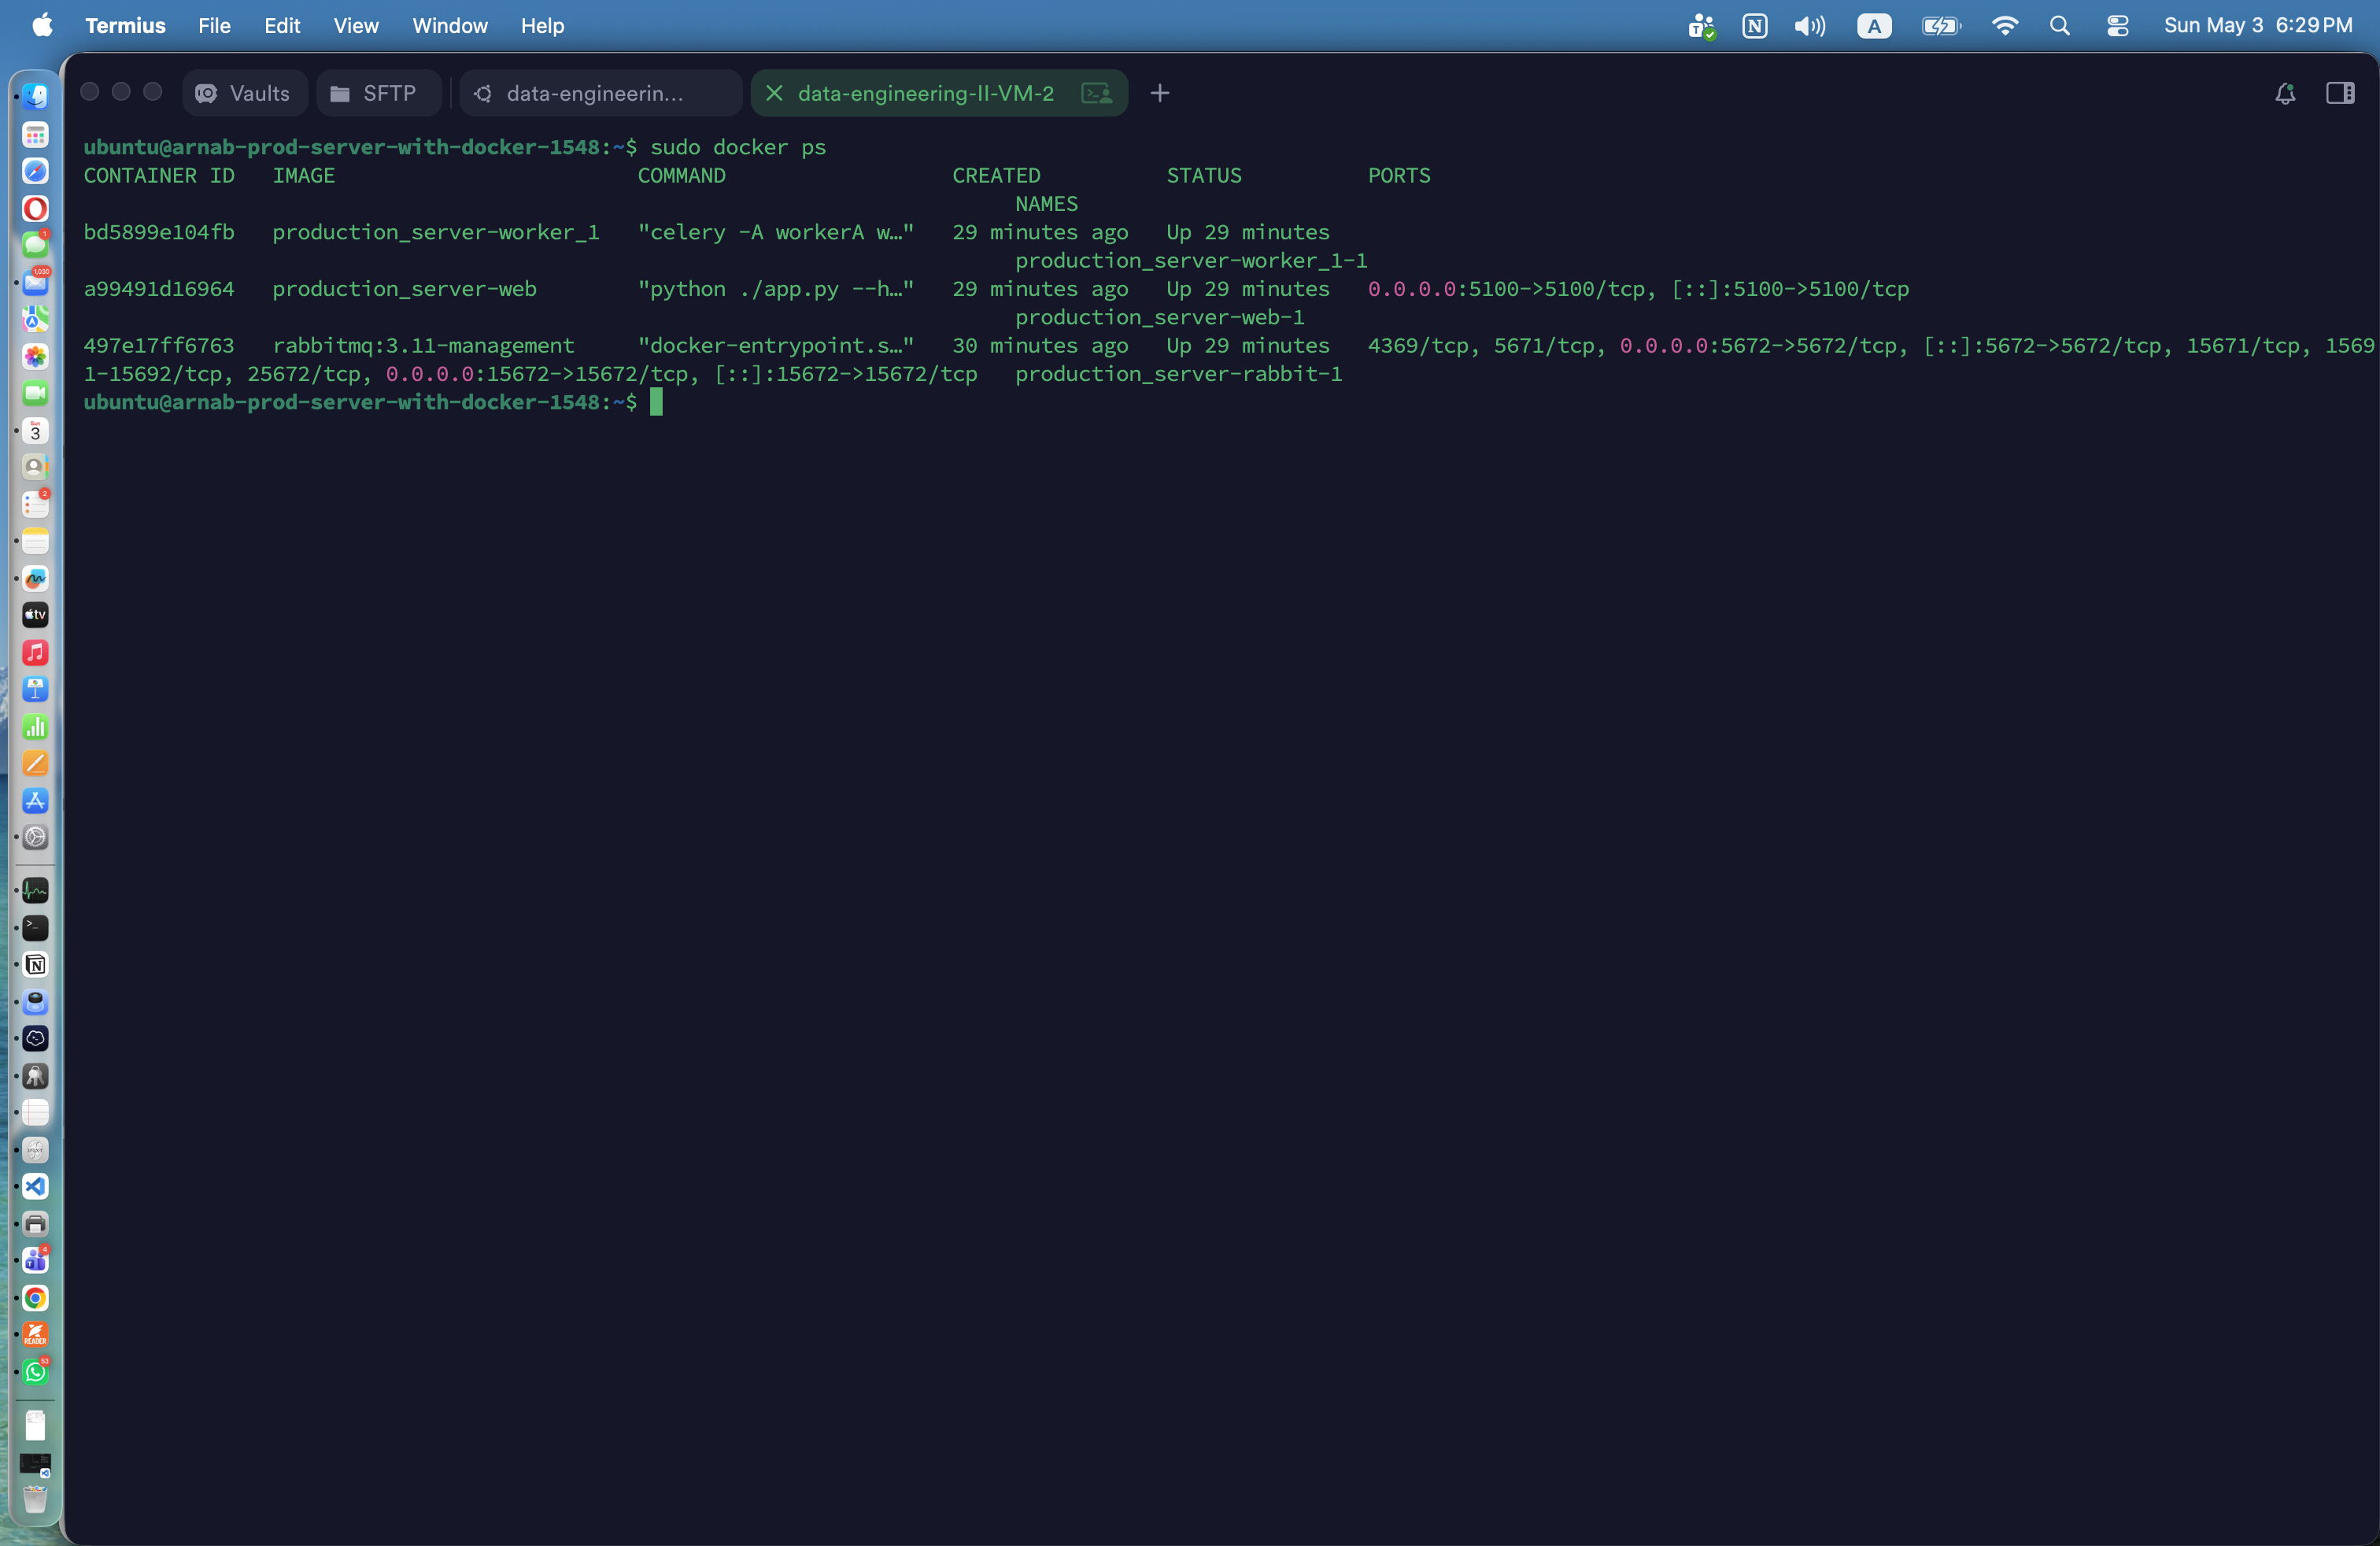
\includegraphics[width=\textwidth]{figure/task-2-docker-ps.png}
  \caption{\texttt{docker ps} output showing the Flask web service, RabbitMQ, and
           a single Celery worker running as separate Docker containers before
           scaling.}
  \label{fig:task2-docker-ps}
\end{figure}

\begin{figure}[htbp]
  \centering
  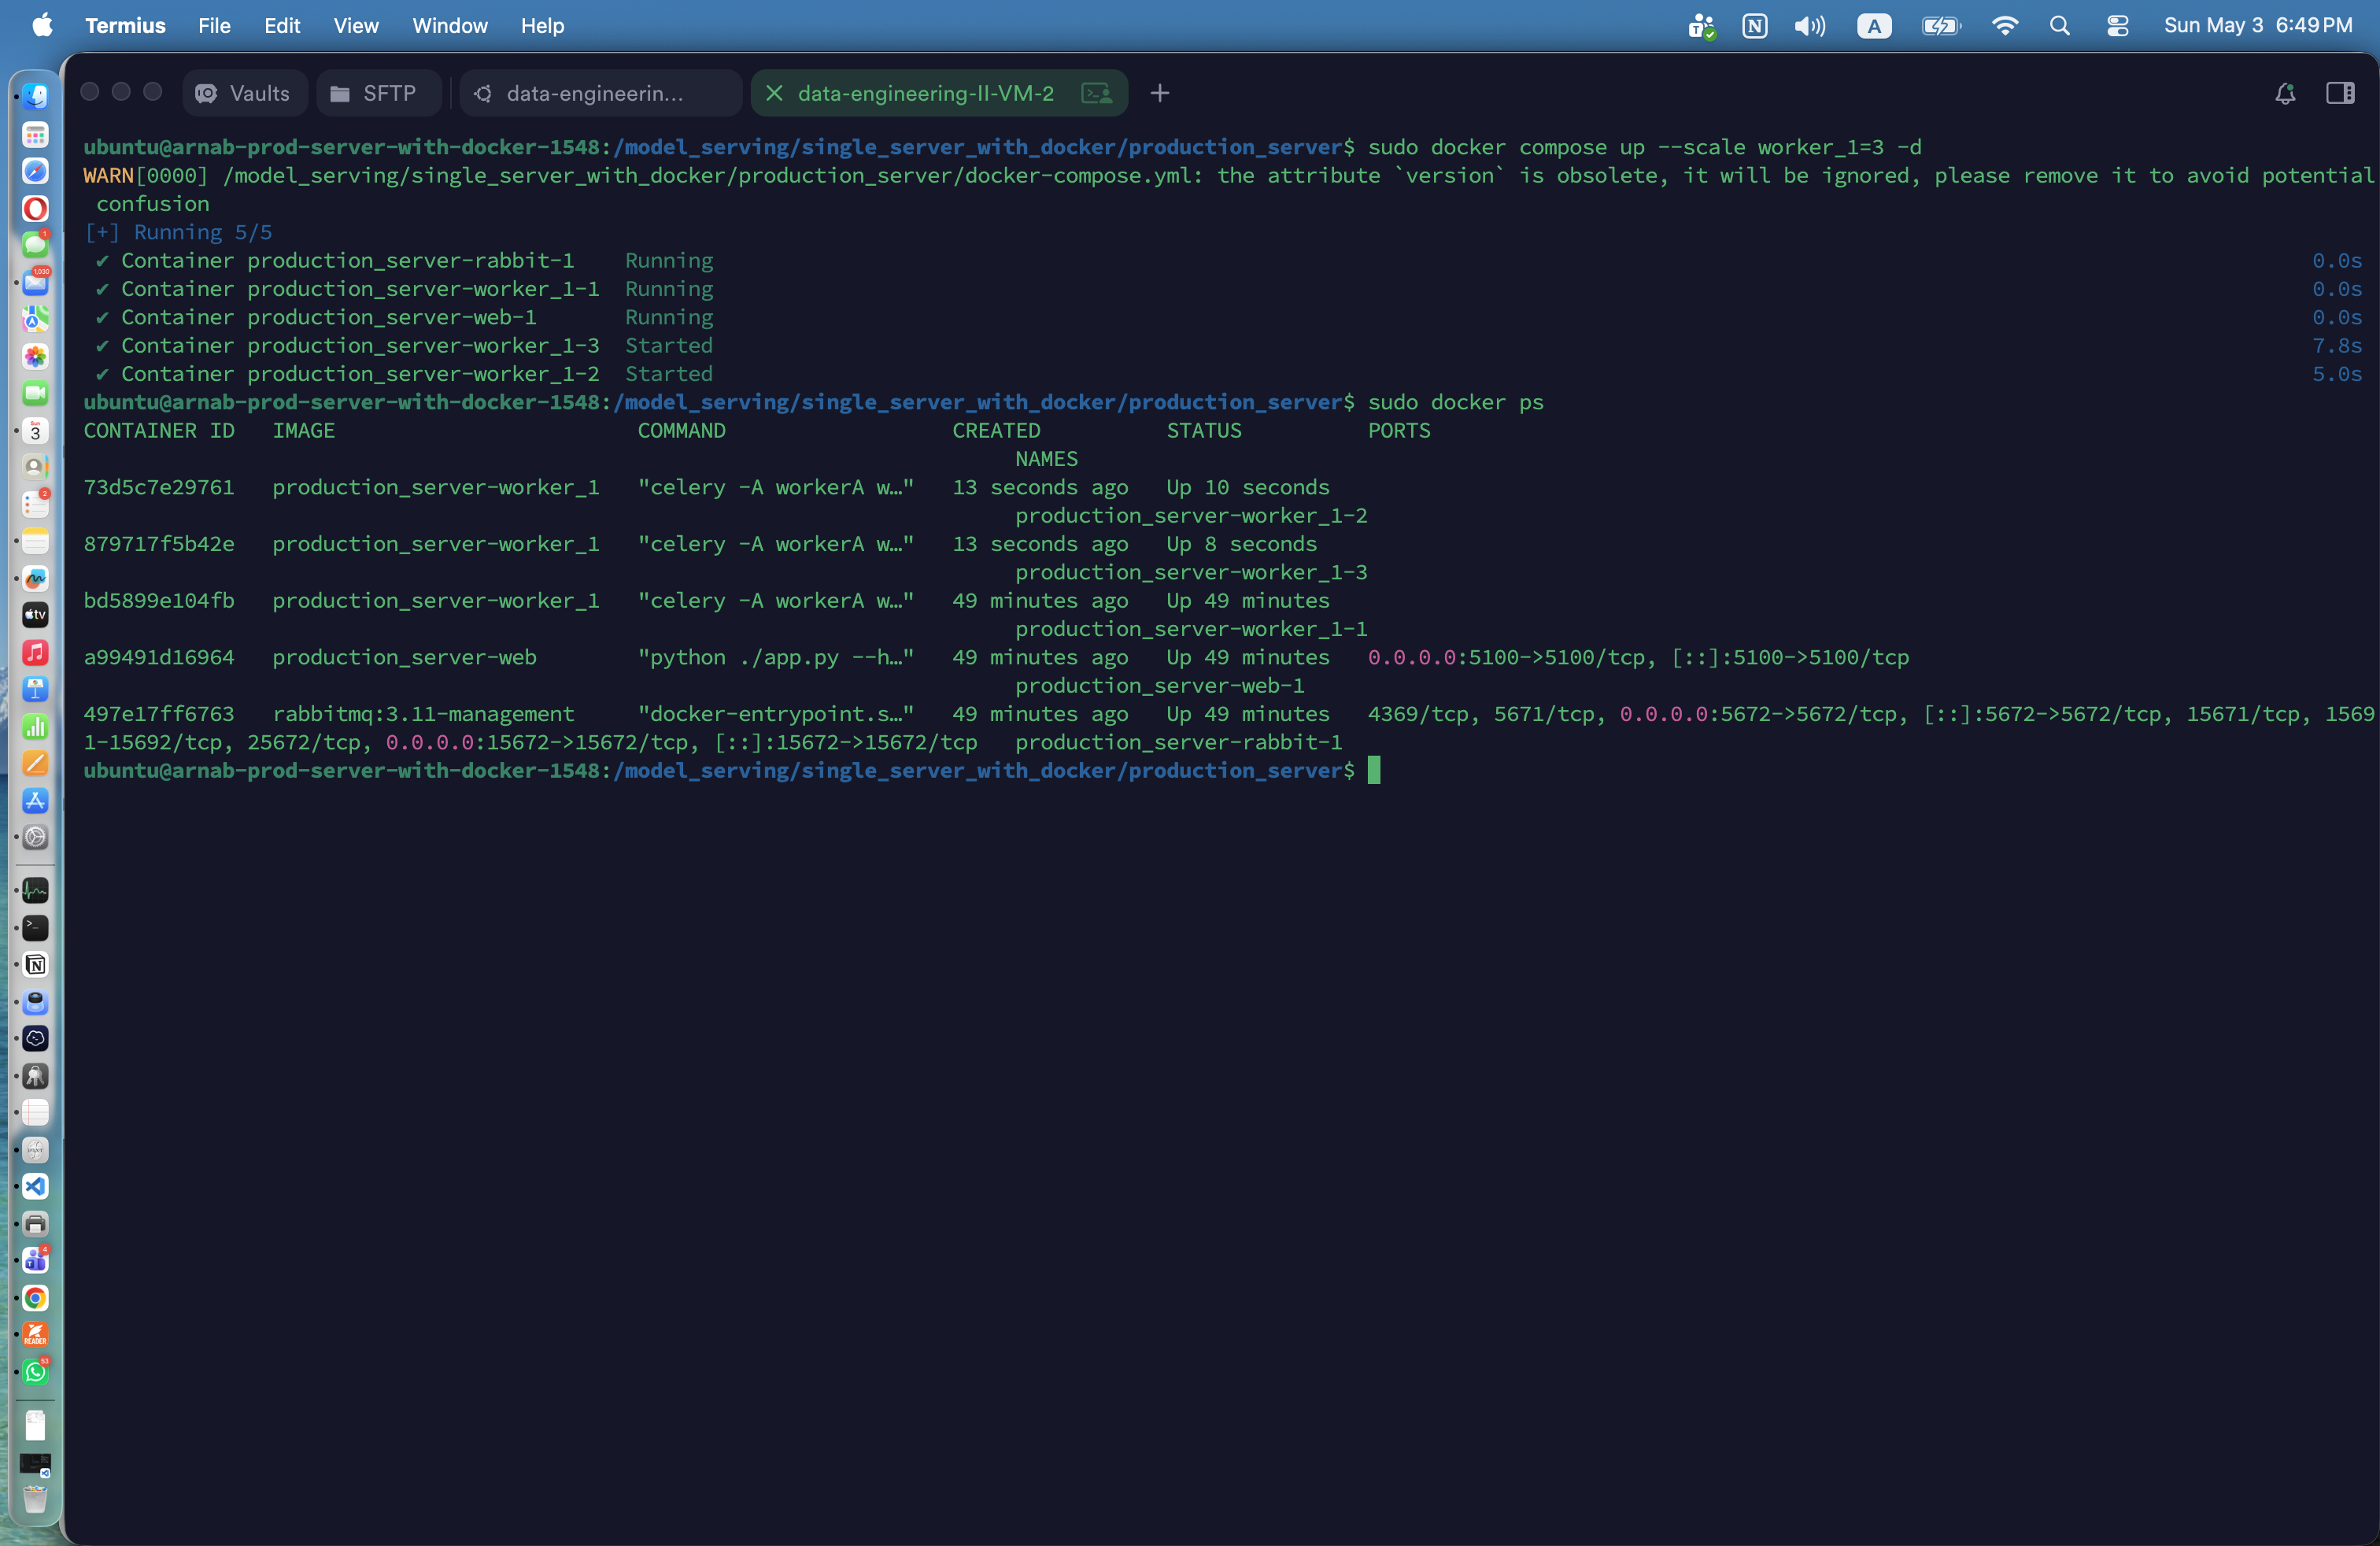
\includegraphics[width=\textwidth]{figure/task-2-docker-ps-scaled.png}
  \caption{\texttt{docker ps} output after running \texttt{docker compose up
           --scale worker\_1=3 -d}. Three Celery worker containers are now running
           alongside the web service and RabbitMQ.}
  \label{fig:task2-docker-ps-scaled}
\end{figure}

\begin{figure}[htbp]
  \centering
  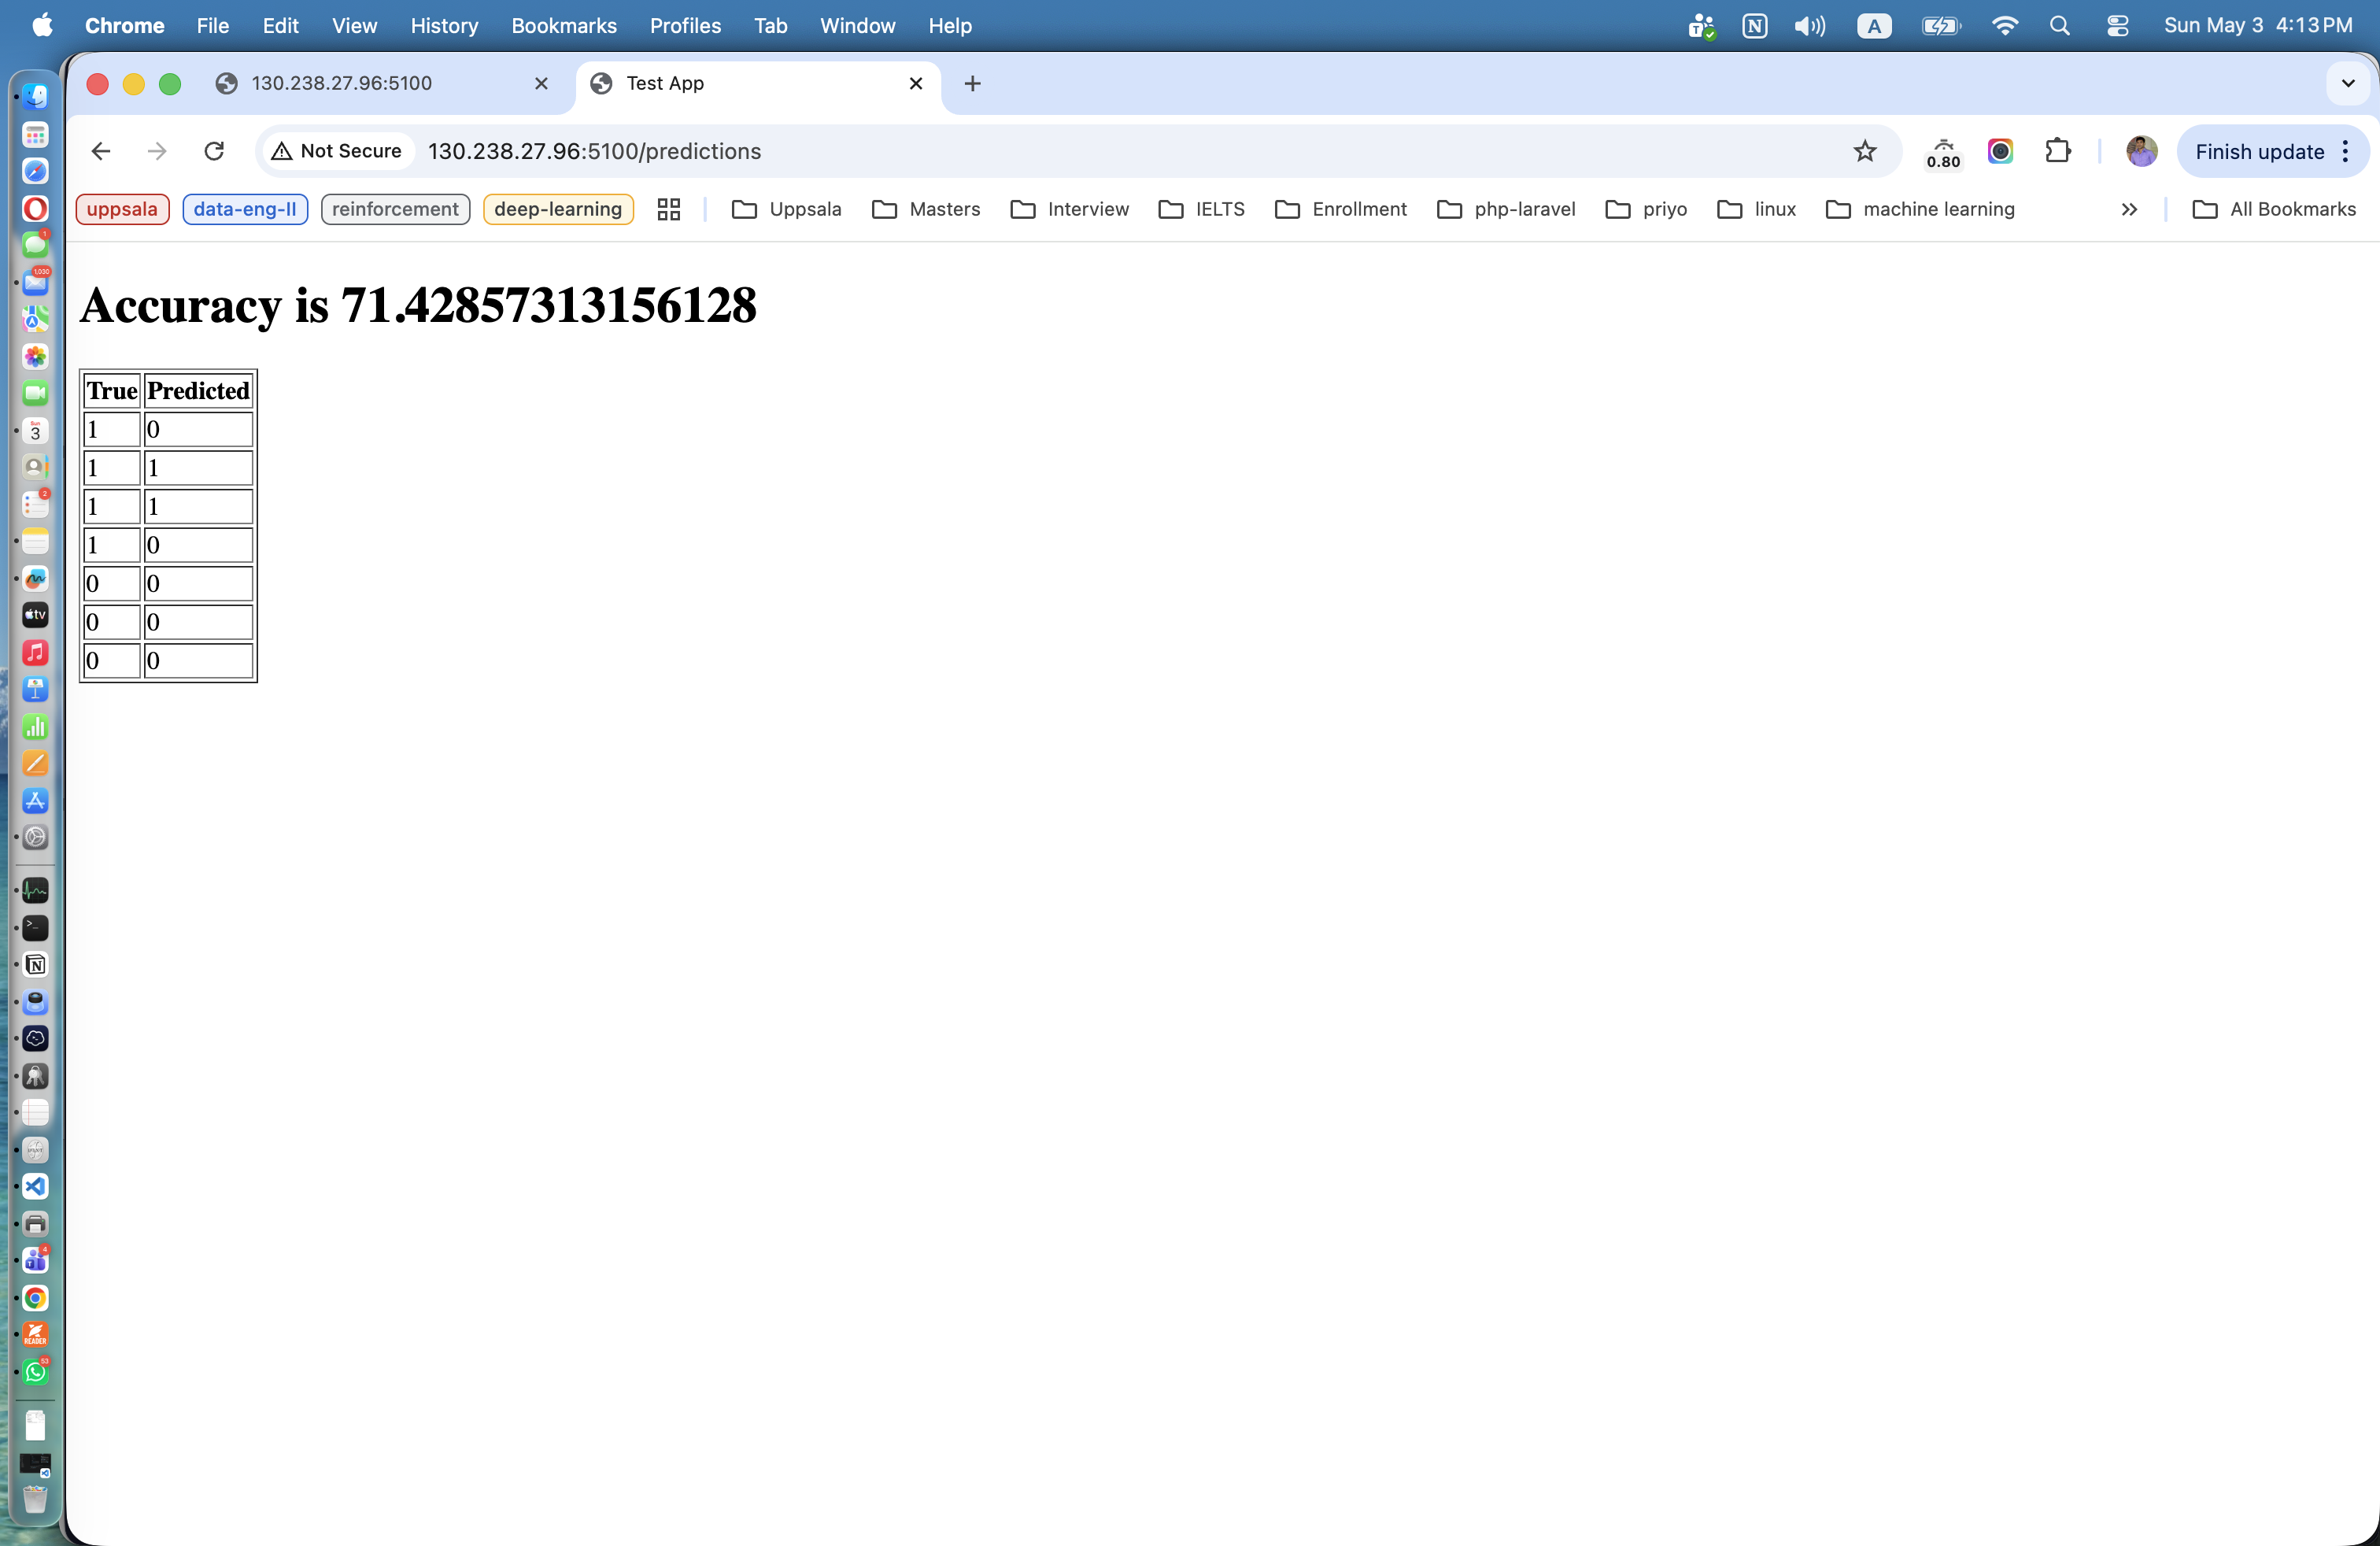
\includegraphics[width=\textwidth]{figure/task-2-predictions.png}
  \caption{Predictions page confirming the application returns correct results
           with three concurrent Celery workers processing tasks in parallel.}
  \label{fig:task2-predictions}
\end{figure}

\newpage

% =============================================================================
\section{Task 3: Deployment of Multiple Servers Using Ansible}
% =============================================================================

\subsection{Overview}

Task 3 requires extending the infrastructure to three virtual machines. A client VM
must manage both a production server and a development server using the OpenStack
Python API to provision them. An Ansible playbook must then configure both servers
simultaneously---handling shared setup tasks once and applying server-specific
configuration in separate plays. This replaces the per-VM CloudInit approach from
Tasks 1 and 2 with a proper configuration management tool that can be re-applied
at any time.

\subsection{Infrastructure}

\begin{itemize}[leftmargin=1.5cm]
  \item \textbf{Client VM}: runs the OpenStack client and Ansible. It creates the
        other two VMs and runs the playbook to configure them.
  \item \textbf{Production server}: runs the Dockerised application from Task 2.
  \item \textbf{Development server}: holds the development code and the model
        training script.
\end{itemize}

\begin{figure}[h!]
  \centering
  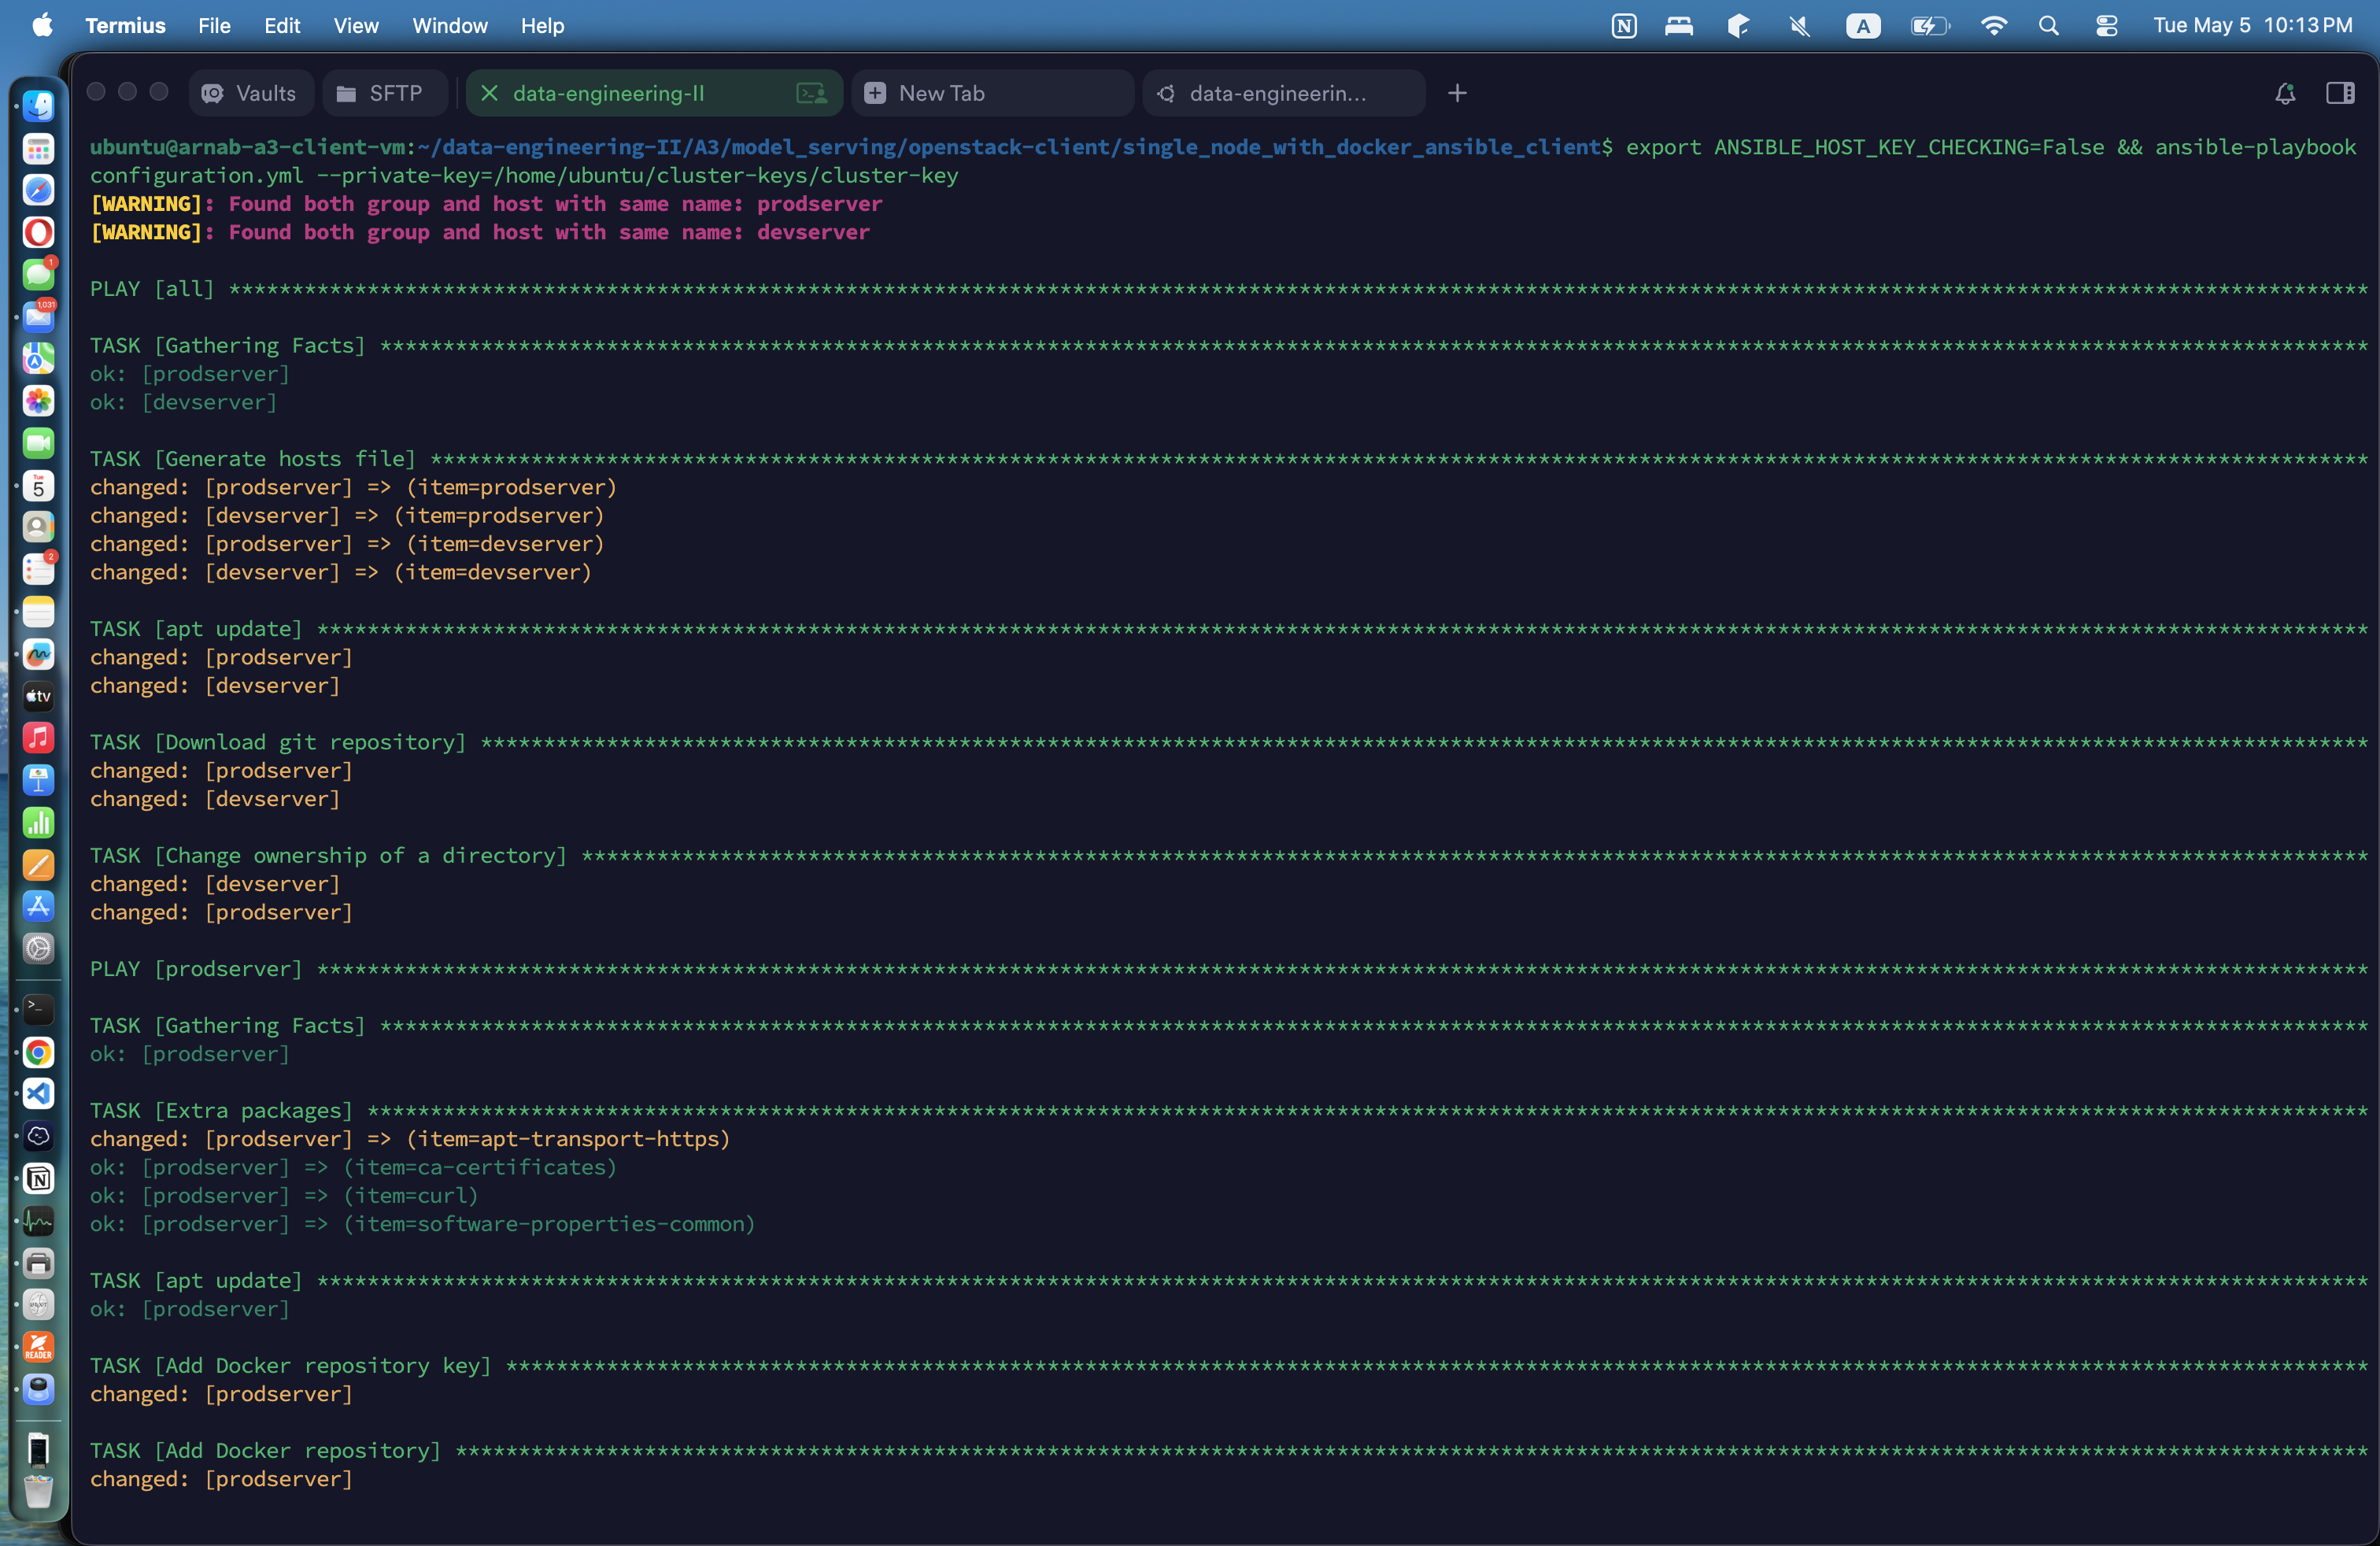
\includegraphics[width=\textwidth]{figure/deployment-multiple-server-using-ansible.png}
  \caption{Deployment architecture for Task 3: Client VM managing production and development servers using Ansible.}
  \label{fig:task3-deployment}
\end{figure}

\subsection{CloudInit Configuration}

Both VMs use a minimal CloudInit file. Each file creates a single
unprivileged user called \texttt{appuser} with passwordless \texttt{sudo} access
and the cluster SSH public key. Ansible then connects over SSH and handles all
further configuration. The production and development files are structurally
identical.

\begin{lstlisting}[style=yaml, caption={prod-cloud-cfg.txt and dev-cloud-cfg.txt (identical structure)}]
#cloud-config

users:
 - name: appuser
   sudo: ALL=(ALL) NOPASSWD:ALL
   home: /home/appuser
   shell: /bin/bash
   ssh_authorized_keys:
     - ssh-rsa AAAA...  # cluster public key (truncated for brevity)

byobu_default: system
\end{lstlisting}

\subsection{Ansible Playbook}

The \texttt{configuration.yml} playbook has three plays. The first play targets
all hosts and handles shared setup. The second targets only the production server
to install Docker and start the application containers. The third targets only
the development server to install the ML packages needed for model training.

\lstinputlisting[style=yaml, caption={configuration.yml}]{../model_serving/openstack-client/single_node_with_docker_ansible_client/configuration.yml}

\subsection{Questions}

\subsubsection*{1. What is the difference between CloudInit and Ansible?}

\textbf{CloudInit} runs once at first boot before SSH is available. It is meant
for bootstrapping: creating users, adding SSH keys, and installing a small set of
packages. It cannot be run again after the VM is created.

\textbf{Ansible} runs from a controller machine over SSH at any point in time.
Playbooks are idempotent, meaning running them several times gives the same result.
Ansible is built for configuration management and can apply changes to many machines
at the same time.

In Task 3, I used CloudInit only for minimal setup. I then used Ansible to connect over SSH and
handle all further configuration.

\subsubsection*{2. Explain the configurations available in dev-cloud-cfg.txt and prod-cloud-cfg.txt files}

Both files share the same structure. Each one creates a single user named
\texttt{appuser} with passwordless \texttt{sudo} access, a \texttt{/bin/bash}
shell, and the cluster SSH public key added to
\texttt{ssh\_authorized\_keys}.
The \texttt{byobu\_default: system} line activates the Byobu terminal
multiplexer for interactive sessions. The files are deliberately minimal
because Ansible handles all further configuration after the VM boots.

\subsubsection*{3. What problem have we solved by using Ansible?}

Ansible solved the problem of configuring multiple machines at the same time.
In Tasks 1 and 2, each VM had its own CloudInit file and was set up independently.
With Ansible, one playbook command configured both the production server and the
development server simultaneously.
Common configuration steps are listed once under \texttt{hosts: all}.
Server-specific steps go in their own section.
If the configuration needs to change, the playbook is updated once and reapplied
to all machines.

\subsubsection*{4. Summary}

In this task, I extended the deployment from a single-server setup to a coordinated
multi-server infrastructure. I provisioned two virtual machines through the
OpenStack Python API from the client VM: the client itself, a production server,
and a development server. I bootstrapped both servers with a minimal CloudInit
file that created the \texttt{appuser} account with SSH access, which allowed
Ansible to connect immediately after boot.

I then ran the Ansible playbook (\texttt{configuration.yml}) with a single command
to configure both servers simultaneously. In the common play, I updated system
packages and cloned the application repository on all hosts. In the production
play, I installed Docker CE and started the application containers via
\texttt{docker compose up -d}, replicating the Task~2 containerised deployment.
In the development play, I installed Python, pip, and the ML packages needed to
train new models with \texttt{neural\_net.py}.

Compared to Tasks 1 and 2, the key improvement I gained is manageability.
When I need to change the configuration, I edit a single playbook file and
reapply it, rather than reprovisioning VMs with updated CloudInit files. The
separation of roles I established---client for orchestration, production for
serving, and development for training---also created the three-VM topology
that the CI/CD pipeline in Task~4 builds directly on.


% =============================================================================
\section{Task 4: CI/CD Using Git Hooks}
% =============================================================================

\subsection{Overview}

Task 4 requires setting up a continuous deployment pipeline using Git Hooks on top of
the multi-server infrastructure from Task 3. A bare Git repository must be created
on the production server, and a \texttt{post-receive} hook must be configured to
automatically deploy new model files to the live application folder whenever
the development server pushes to the master branch. The goal is to eliminate any
manual file copying or service restart from the model-update workflow.

\subsection{Architecture}

The pipeline uses the same three VMs from Task 3:

\begin{itemize}[leftmargin=1.5cm]
  \item \textbf{Development server}: trains a new model with \texttt{neural\_net.py}
        and pushes the model files to the production server over Git.
  \item \textbf{Production server}: has a bare Git repository at
        \texttt{/home/appuser/my\_project}. The \texttt{post-receive} hook copies
        new files to the live application folder on every push.
  \item \textbf{Client VM}: used in Task~3 to provision and configure the production
        and development servers via Ansible. It is not part of the ongoing push
        pipeline once the infrastructure is in place.
\end{itemize}

\begin{center}
  \texttt{Dev Server} $\xrightarrow{\text{git push (SSH)}}$
  \texttt{Prod bare repo} $\xrightarrow{\text{post-receive hook}}$
  \texttt{/model\_serving/ci\_cd/production\_server}
\end{center}

\begin{figure}[h!]
  \centering
  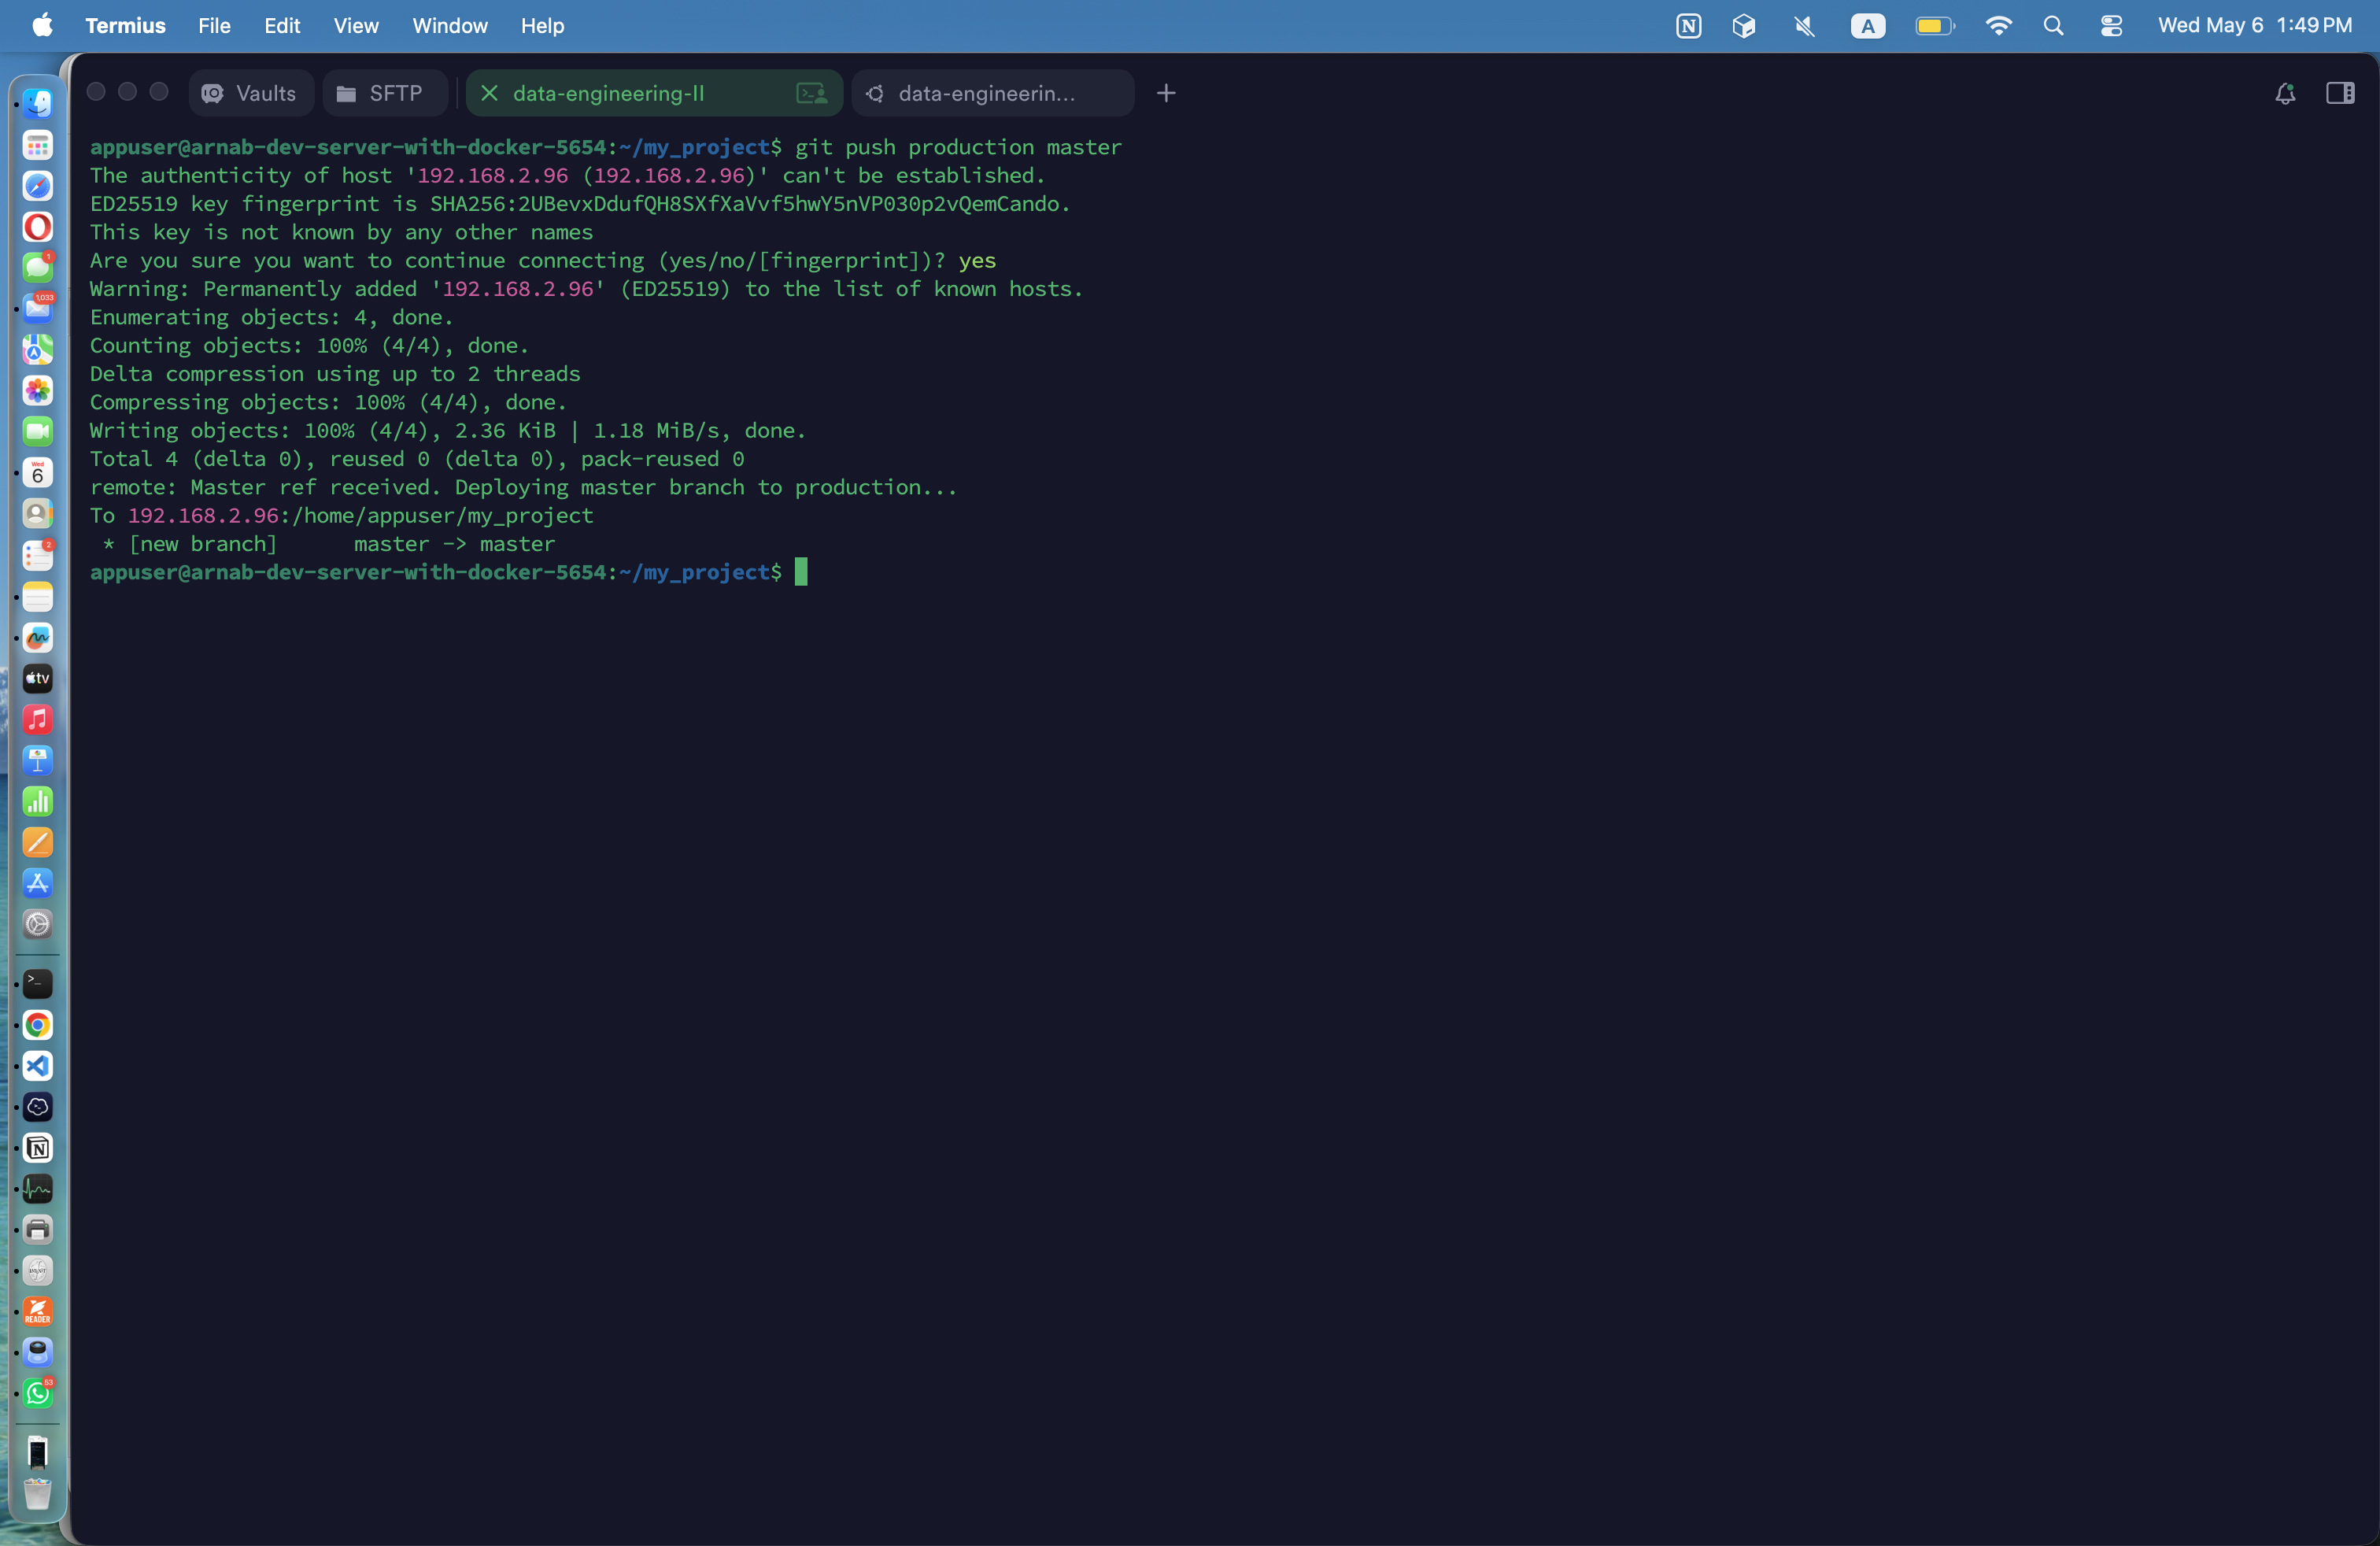
\includegraphics[width=\textwidth]{figure/deployment-to-production-using-git-hook.png}
  \caption{Deployment pipeline: development server pushes model files to production server via Git, triggering the post-receive hook for automated deployment.}
  \label{fig:task4-git-hook-pipeline}
\end{figure}

\subsection{The post-receive Hook}

The hook file is at
\texttt{/home/appuser/my\_project/hooks/post-receive} on the production server:

\begin{lstlisting}[style=shell, caption={post-receive Git hook on the production server}]
#!/bin/bash
while read oldrev newrev ref
do
  if [[ $ref =~ .*/master$ ]];
  then
    echo "Master ref received. Deploying master branch to production..."
    sudo git --work-tree=/model_serving/ci_cd/production_server \
             --git-dir=/home/appuser/my_project checkout -f
  else
    echo "Ref $ref successfully received. Doing nothing: only the master \
branch may be deployed on this server."
  fi
done
\end{lstlisting}

The hook reads each pushed branch name. If the branch is \texttt{master}, it runs
\texttt{git checkout -f} with \texttt{--work-tree} to copy the pushed files into
the live application folder. Old model files are replaced. If any other branch is
pushed, the hook prints a message and does nothing.

\subsection{Running the Pipeline}

\begin{lstlisting}[style=shell, caption={Initial push from the development server}]
# On the development server
mkdir /home/appuser/my_project && cd /home/appuser/my_project
git init
cp /model_serving/ci_cd/development_server/model* .
git add .
git commit -m "initial model"
git remote add production appuser@<PROD-IP>:/home/appuser/my_project
git push production master
\end{lstlisting}

\begin{lstlisting}[style=shell, caption={Updating the model and pushing to production}]
# Train a new model on the development server
sudo python3 /model_serving/ci_cd/development_server/neural_net.py

# Copy new model files to the git working directory
cp /model_serving/ci_cd/development_server/model* /home/appuser/my_project/

# Commit and push
cd /home/appuser/my_project
git add .
git commit -m "updated model"
git push production master
\end{lstlisting}

The \texttt{neural\_net.py} script trains a new model and saves updated model files.
When pushed, the \texttt{post-receive} hook automatically deploys these new files
to production. The expected output confirms the hook ran:

\begin{lstlisting}[style=shell]
remote: Master ref received. Deploying master branch to production...
To 192.168.x.x:/home/appuser/my_project
   c20d19e..666ca0c  master -> master
\end{lstlisting}

\subsection{Questions}

\subsubsection*{1. What are Git hooks? Explain the post-receive script.}

Git hooks are shell scripts that Git runs at certain points in the workflow. They
are stored in the \texttt{hooks/} folder of a repository. Each hook has a fixed
name that matches the event it listens to.

The \texttt{post-receive} script in this task runs on the production server after a
push is fully received. It reads each pushed branch. If the branch is
\texttt{master}, it runs:

\begin{lstlisting}[style=shell]
sudo git --work-tree=/model_serving/ci_cd/production_server \
         --git-dir=/home/appuser/my_project checkout -f
\end{lstlisting}

This copies the files from the push into the live folder, replacing the current
model files. If any other branch is pushed, the hook only prints a message and
stops. This makes sure only \texttt{master} commits reach production.

\subsubsection*{2. Why is the bare Git repository needed on the production server?}

A bare repository stores only the Git object database with no working tree.
It serves as the remote that the development server pushes to.
A regular repository cannot accept a push to its active branch because Git
cannot safely update the working tree during the push.
A bare repository has no active branch and no working files, so it always
accepts pushes. After the push completes, the \texttt{post-receive} hook copies
files to a separate live folder using \texttt{--work-tree}.
This separation keeps Git storage and the running application files in
different locations.

\subsubsection*{3. Four Git hooks and their functionalities.}

\begin{enumerate}[leftmargin=1.5cm]
  \item \textbf{pre-commit}: runs before a commit is saved. It is often used to
        run linters or tests. If it exits with an error, the commit is cancelled.
  \item \textbf{commit-msg}: runs after a commit message is written. It can check
        that the message follows a required format, such as including a ticket
        number.
  \item \textbf{pre-receive}: runs on the server before any branch is updated. It
        can reject a push based on rules such as file size or branch naming.
  \item \textbf{post-receive}: runs on the server after all branches are updated.
        It is used to trigger deployments, send alerts, or update build status---as
        shown in this task.
\end{enumerate}

\subsubsection*{4. Kubernetes deployment diagram for the multi-server setup.}

I could run the same application from Task 3 in Kubernetes.
A \textbf{Deployment} manages the Flask web pods and exposes them via a
\textbf{Service} of type \texttt{LoadBalancer}.
RabbitMQ runs in a \textbf{StatefulSet} behind a headless \textbf{Service}.
The Celery workers run in a separate \textbf{Deployment} that can be scaled
independently.
A \textbf{ConfigMap} stores non-secret settings like the RabbitMQ hostname.
A \textbf{Secret} stores credentials.
Both web pods and worker pods mount the same \textbf{PersistentVolumeClaim}
to access model files.

\begin{figure}[h!]
  \centering
  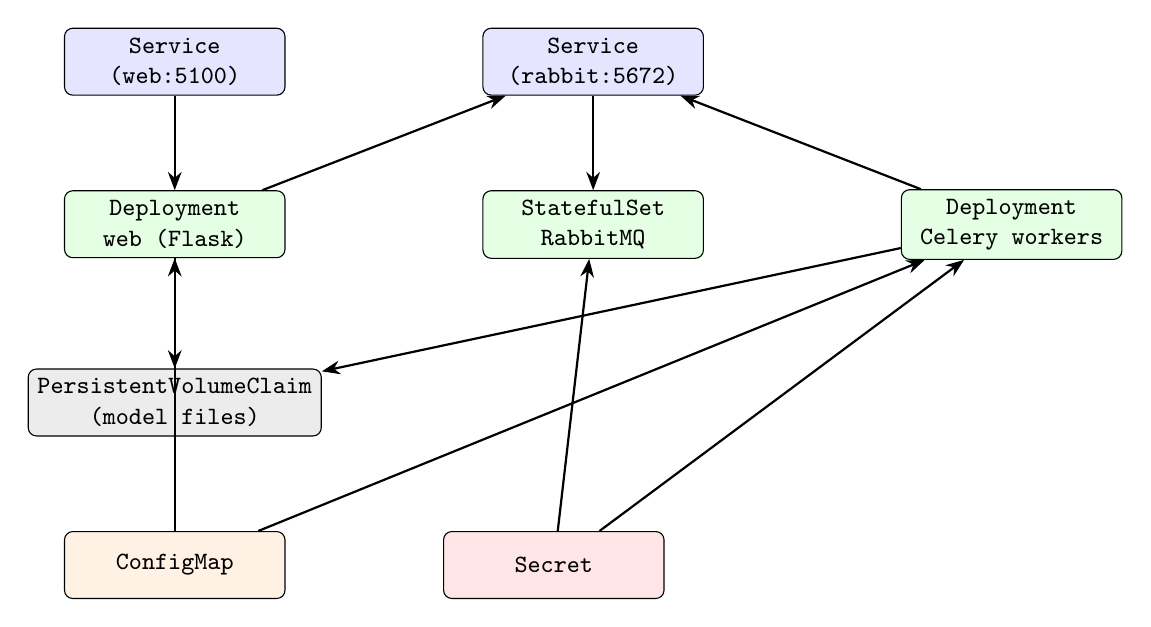
\begin{tikzpicture}[
      node distance=1.2cm and 2.0cm,
      box/.style={rectangle, draw, rounded corners=3pt,
                  minimum width=2.8cm, minimum height=0.85cm,
                  font=\small\ttfamily, align=center},
      svc/.style={box, fill=blue!10},
      dep/.style={box, fill=green!10},
      cfg/.style={box, fill=orange!10},
      sec/.style={box, fill=red!10},
      pvc/.style={box, fill=gray!15},
      arr/.style={-Stealth, thick},
    ]
    \node[svc]  (web-svc)  {Service\\(web:5100)};
    \node[dep]  (web-dep)  [below=of web-svc]   {Deployment\\web (Flask)};
    \node[svc]  (rmq-svc)  [right=2.5cm of web-svc] {Service\\(rabbit:5672)};
    \node[dep]  (rmq-dep)  [below=of rmq-svc]   {StatefulSet\\RabbitMQ};
    \node[dep]  (wkr-dep)  [right=2.5cm of rmq-dep] {Deployment\\Celery workers};
    \node[pvc]  (pvc)      [below=1.4cm of web-dep] {PersistentVolumeClaim\\(model files)};
    \node[cfg]  (cm)       [below=of pvc]            {ConfigMap};
    \node[sec]  (secret)   [right=2cm of cm]          {Secret};

    \draw[arr] (web-svc) -- (web-dep);
    \draw[arr] (rmq-svc) -- (rmq-dep);
    \draw[arr] (web-dep) -- (rmq-svc);
    \draw[arr] (wkr-dep) -- (rmq-svc);
    \draw[arr] (web-dep) -- (pvc);
    \draw[arr] (wkr-dep) -- (pvc);
    \draw[arr] (cm)      -- (web-dep);
    \draw[arr] (cm)      -- (wkr-dep);
    \draw[arr] (secret)  -- (rmq-dep);
    \draw[arr] (secret)  -- (wkr-dep);
  \end{tikzpicture}
  \caption{Kubernetes deployment diagram: Flask web Deployment behind a Service,
           RabbitMQ StatefulSet with headless Service, Celery worker Deployment,
           shared PersistentVolumeClaim for model files, ConfigMap and Secret for
           configuration and credentials.}
  \label{fig:k8s-diagram}
\end{figure}

\subsubsection*{5. Summary}

In this task, I completed the continuous deployment pipeline for the model serving
application. I combined the multi-server infrastructure from Task~3 with a
Git-based deployment mechanism. This created an end-to-end workflow where a
retrained model is live in production within seconds of a \texttt{git push},
with no manual file copying or service restart needed.

I set up the pipeline using only Git and SSH---both of which were already present
from Task~3. I created a bare repository on the production server as the deployment
target and wrote the \texttt{post-receive} hook as the deployment agent. When I push new model files from the development server to the master branch,
the hook is triggered immediately. It runs \texttt{git checkout -f} with the
\texttt{--work-tree} flag pointing to the live application folder. This replaces
the old model files with the new ones.
The entire deployment happens server-side with no further action needed from me.

I verified the pipeline end-to-end with a before-and-after test. Before the push,
I confirmed the predictions page showed results from the original model. I then
trained a new model by running \texttt{neural\_net.py} on the development server,
copied the updated files into the local Git working directory, committed, and
pushed to the production bare repository. The hook deployed the new model files
automatically, and I confirmed the predictions page reflected the updated model
output, showing that the new \texttt{model.h5} and \texttt{model.json} were
picked up by the running Celery worker.

I found this approach lightweight and effective for a single-server production
setup. The main limitation I identified is that file replacement is not atomic:
a worker reading the model during a push could briefly encounter an inconsistent
state. In a production environment I would address this with a blue-green
deployment or a container image swap, but for this task the simple file-copy
approach demonstrated the core CI/CD concept clearly and proved reliable in
practice.

\begin{figure}[htbp]
  \centering
  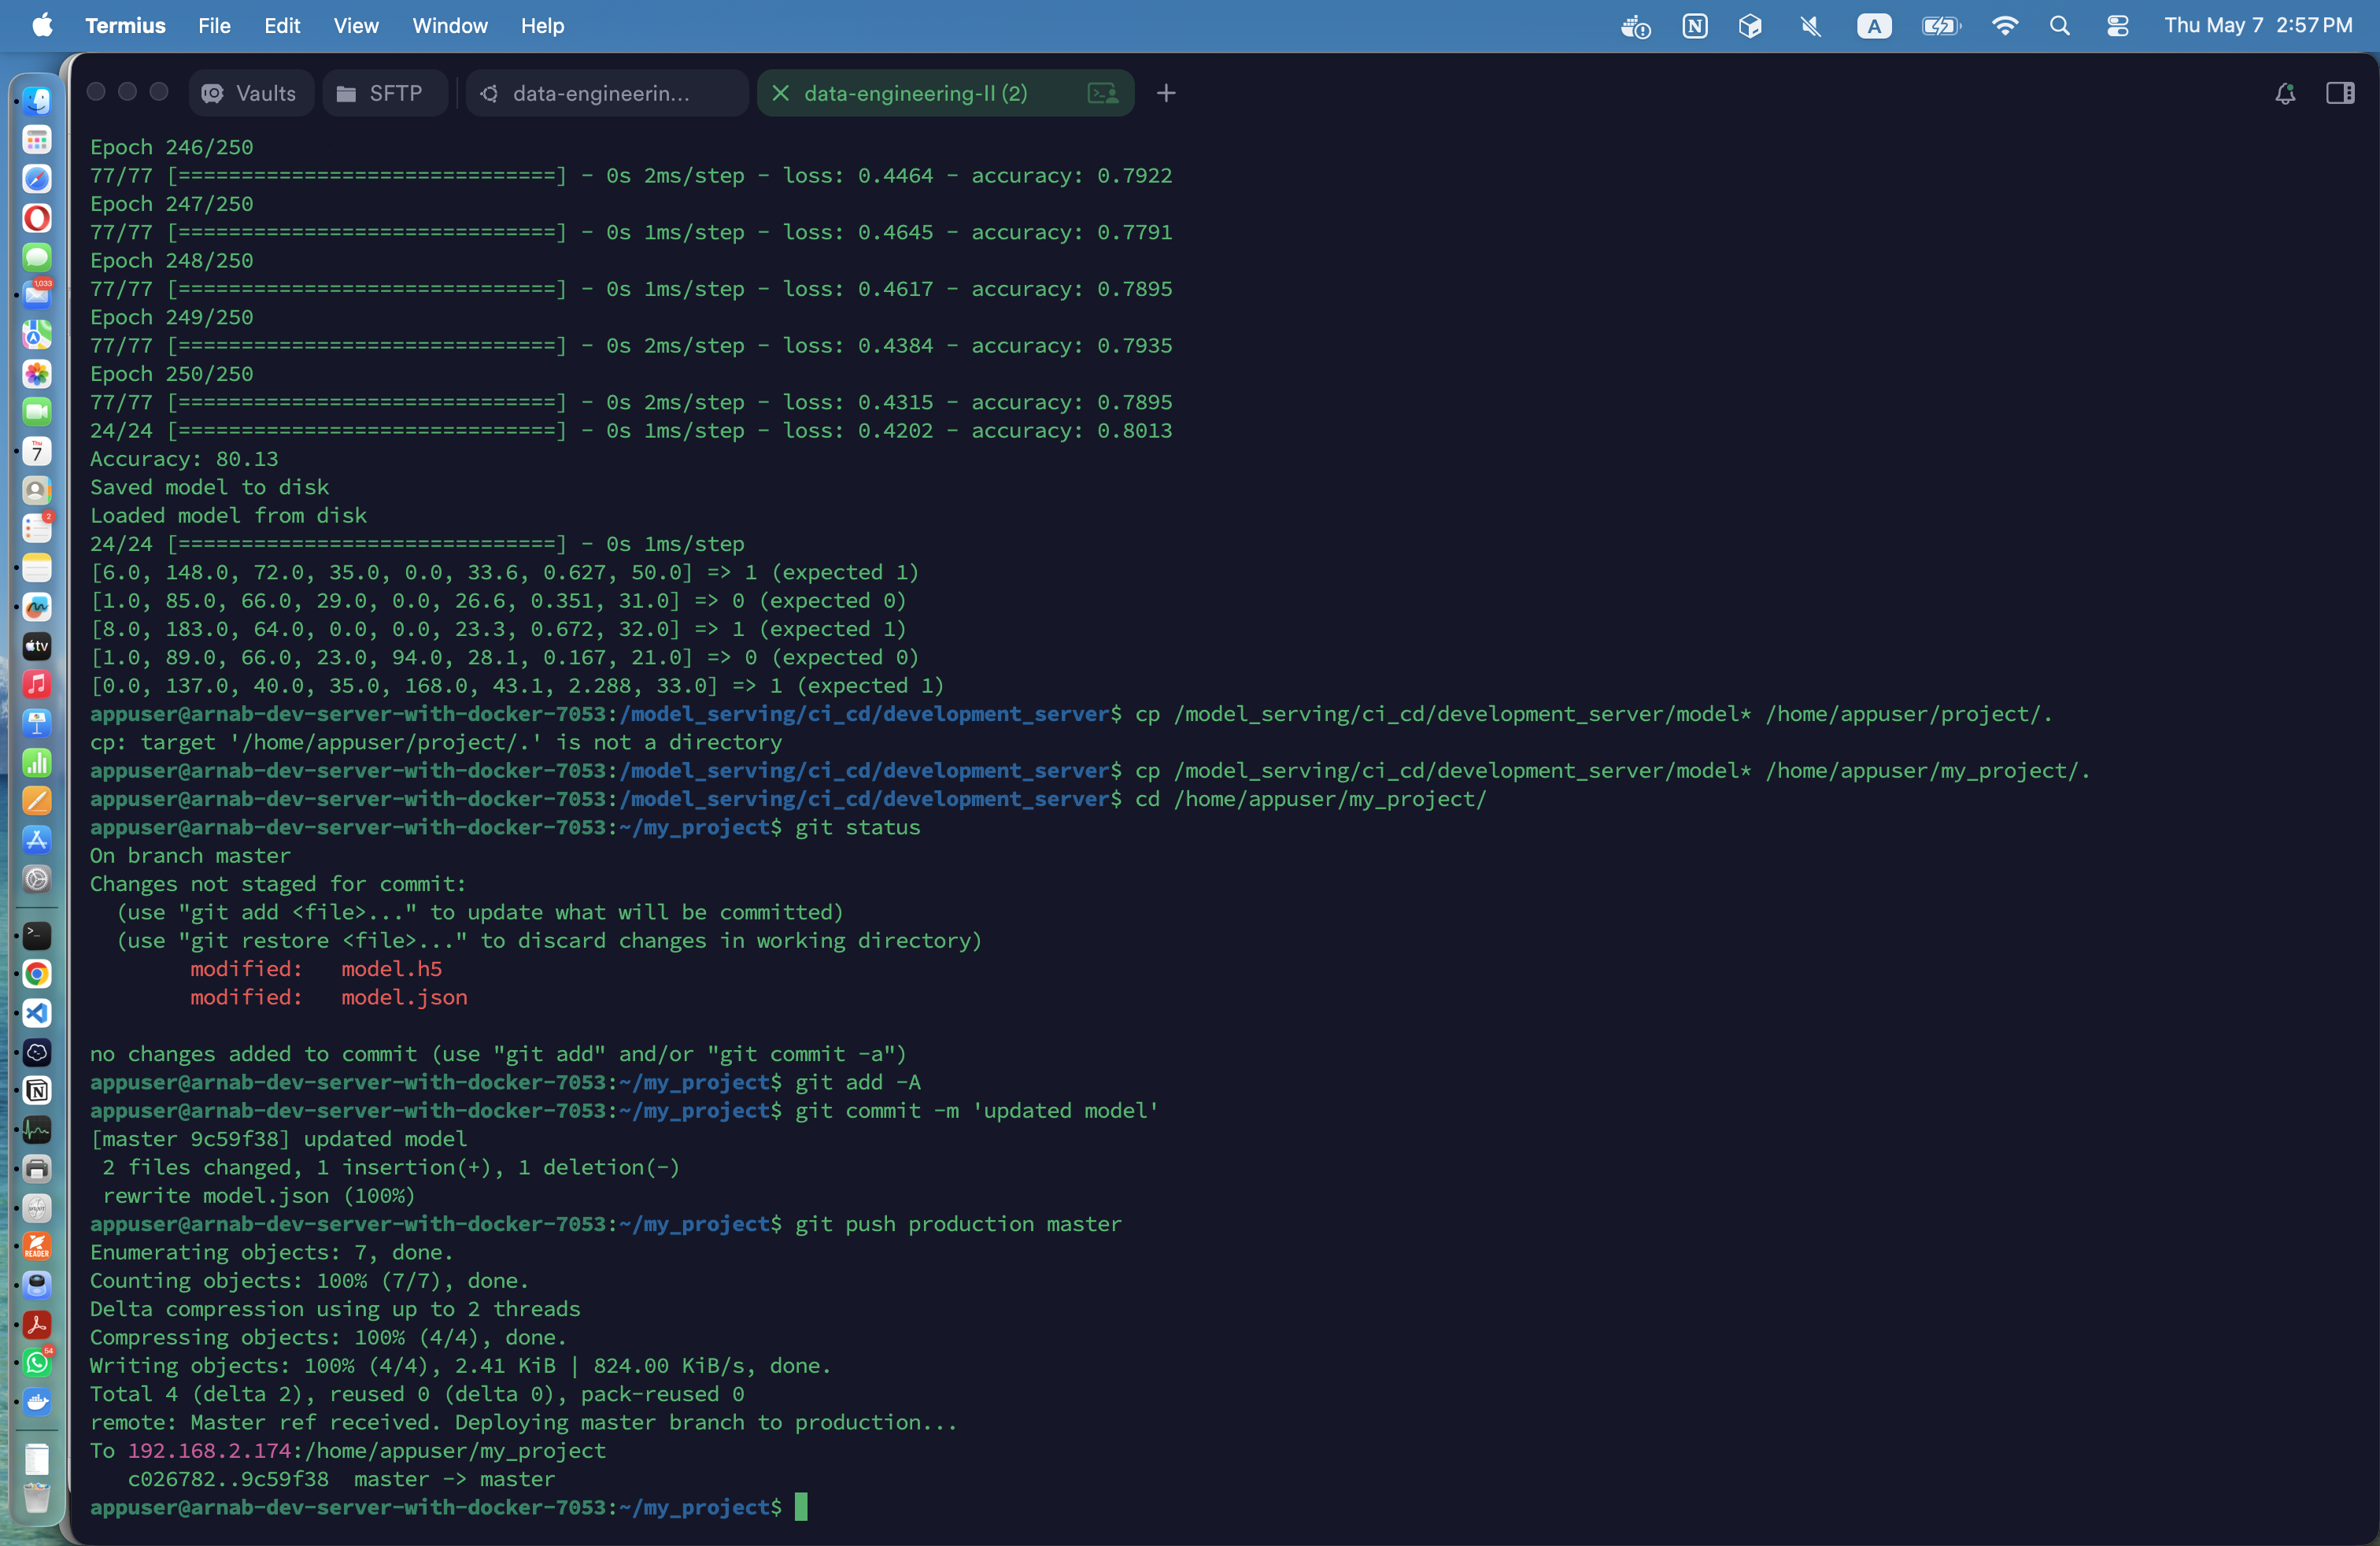
\includegraphics[width=\textwidth]{figure/task-4-git-push.png}
  \caption{Terminal output of \texttt{git push production master} confirming that
           the \texttt{post-receive} hook ran and deployed the updated model files
           to the live application folder on the production server.}
  \label{fig:task4-push}
\end{figure}

\begin{figure}[htbp]
  \centering
  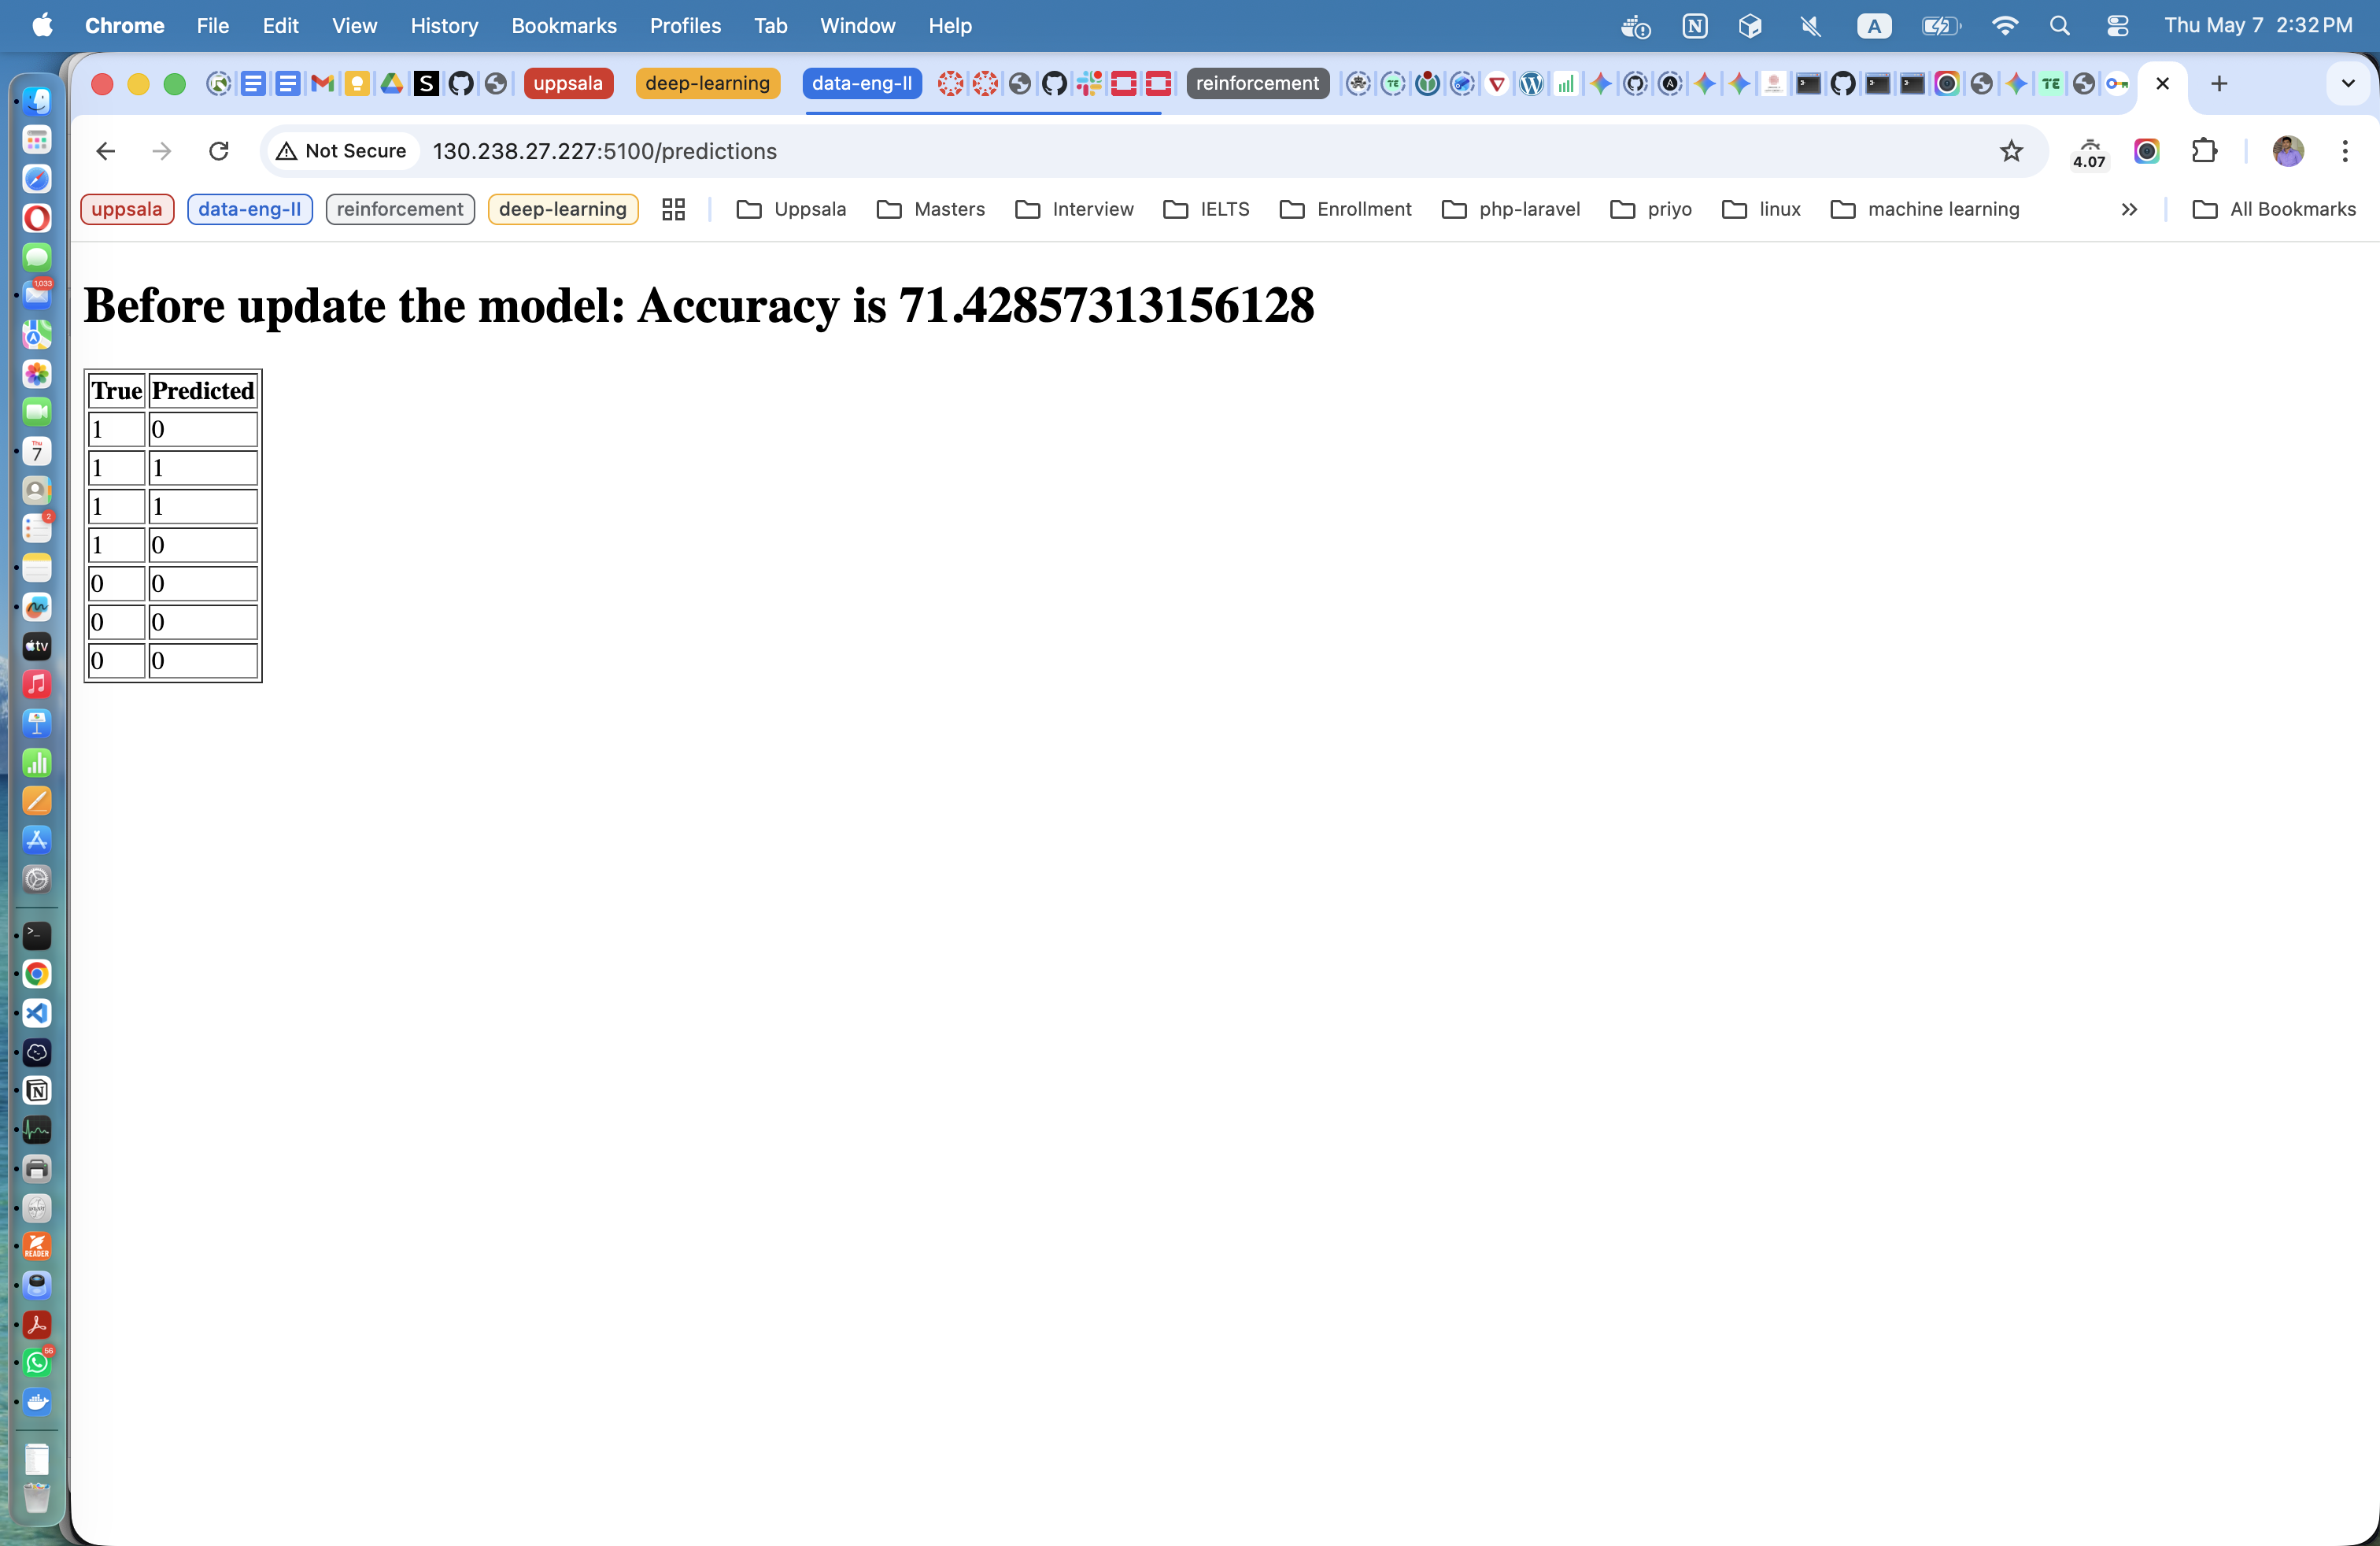
\includegraphics[width=\textwidth]{figure/task-4-before-update-predictions.png}
  \caption{Predictions page before the CI/CD pipeline push, showing inference
           results from the original trained model.}
  \label{fig:task4-before-predictions}
\end{figure}

\begin{figure}[htbp]
  \centering
  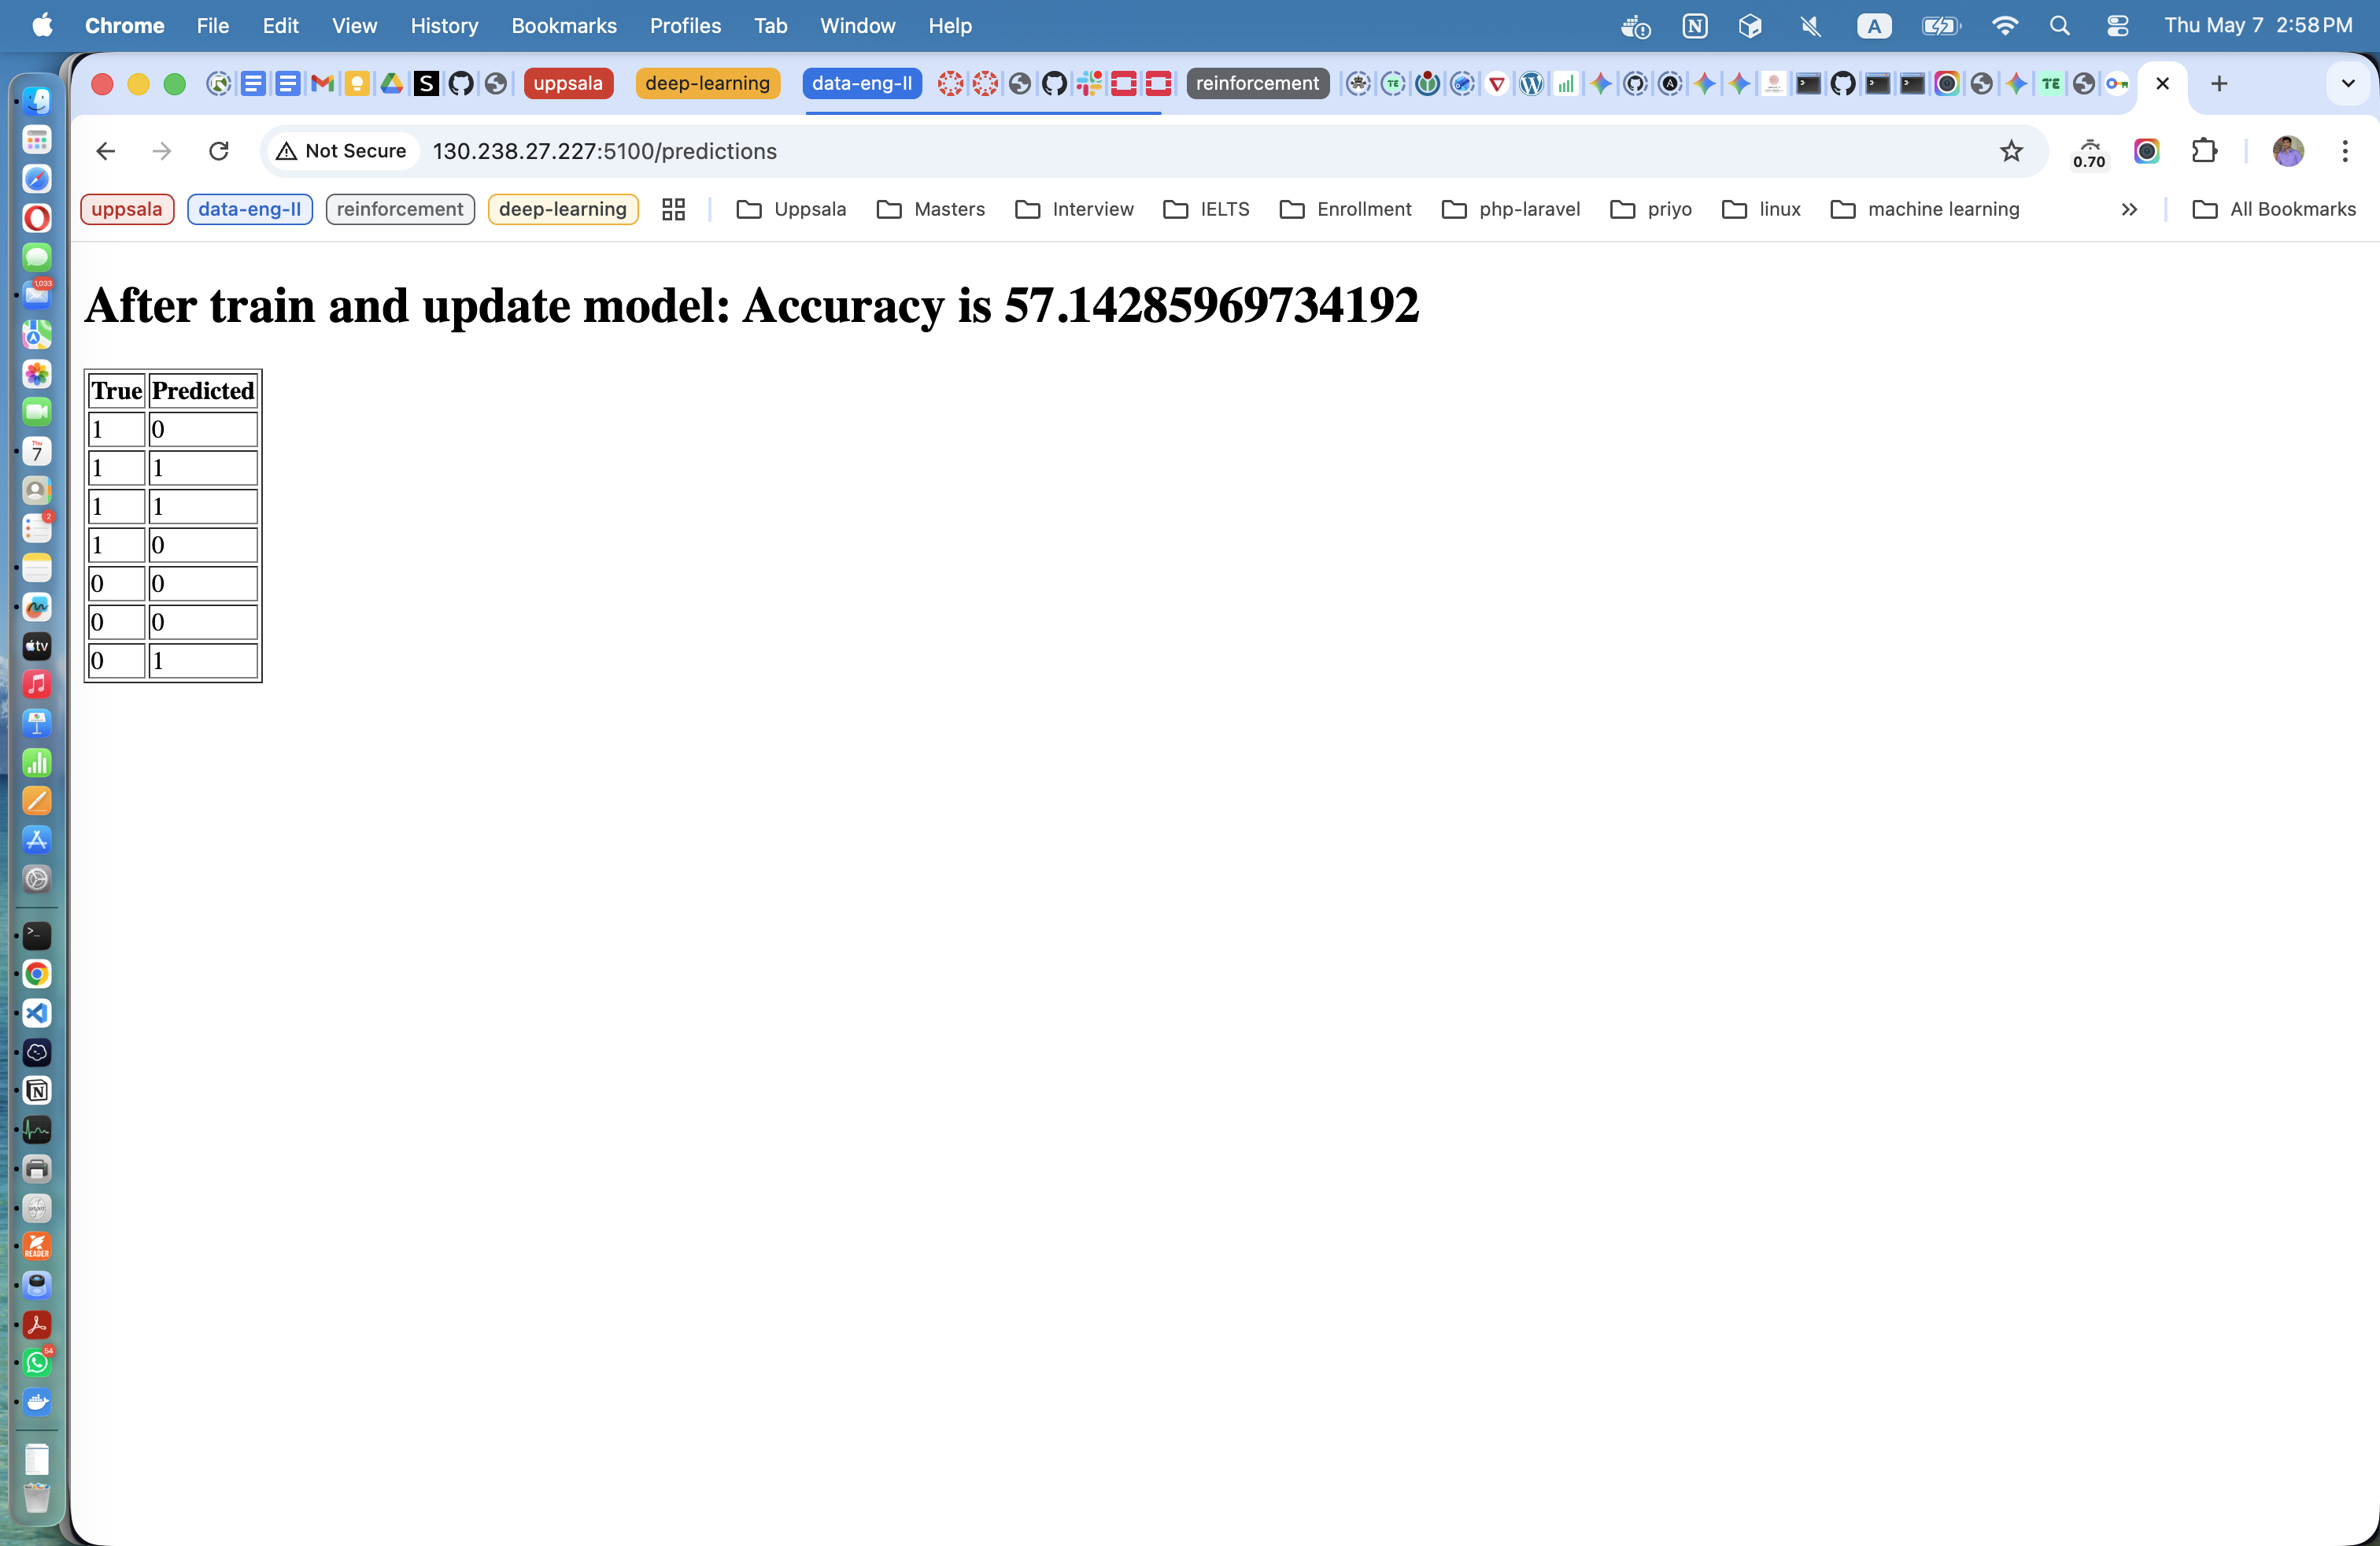
\includegraphics[width=\textwidth]{figure/task-4-updated-predictions.png}
  \caption{Predictions page after the CI/CD push, showing updated inference
           results from the retrained model deployed automatically via the
           \texttt{post-receive} hook.}
  \label{fig:task4-predictions}
\end{figure}

\newpage

% =============================================================================
\section{Conclusion}
% =============================================================================

This assignment demonstrated a progressive path toward reliable cloud deployment
and continuous deployment. Task 1 established basic manual deployment with CloudInit.
Task 2 improved this with Docker containers, providing isolation and easy scaling.
Task 3 scaled further with Ansible, managing multiple servers from a single
control point. Task 4 completed the cycle by automating model updates through
a Git-based CI/CD pipeline.

Together, these tasks show how modern infrastructure tools address real deployment
challenges: reproducibility, scalability, configuration management, and automation.
The progression from single-server CloudInit deployment to multi-server Ansible
orchestration with automated CI/CD demonstrates industry best practices for
production infrastructure.

\end{document}

